%File: formatting-instruction.tex
\documentclass[letterpaper]{article} % DO NOT CHANGE THIS
\usepackage{aaai24}  % DO NOT CHANGE THIS
\usepackage{times}  % DO NOT CHANGE THIS
\usepackage{helvet}  % DO NOT CHANGE THIS
\usepackage{courier}  % DO NOT CHANGE THIS
\usepackage[hyphens]{url}  % DO NOT CHANGE THIS
\usepackage{graphicx} % DO NOT CHANGE THIS
\urlstyle{rm} % DO NOT CHANGE THIS
\def\UrlFont{\rm}  % DO NOT CHANGE THIS
\usepackage{natbib}  % DO NOT CHANGE THIS AND DO NOT ADD ANY OPTIONS TO IT
\usepackage{caption} % DO NOT CHANGE THIS AND DO NOT ADD ANY OPTIONS TO IT
\frenchspacing  % DO NOT CHANGE THIS
\setlength{\pdfpagewidth}{8.5in}  % DO NOT CHANGE THIS
\setlength{\pdfpageheight}{11in}  % DO NOT CHANGE THIS
\usepackage{algorithm}
% \usepackage{algorithmic}
\usepackage{multirow}
\usepackage{makecell}
\usepackage{pifont}
\usepackage{bbding}
\usepackage{amsmath}
\usepackage{amssymb}
\usepackage{algpseudocode}
\usepackage{booktabs}
\usepackage{amstext}
\usepackage{bm}
% \usepackage{subfigure}
\newcommand{\eg}{\textit{e}.\textit{g}.}
\usepackage{enumitem}
\usepackage[table]{xcolor}

\usepackage{url}            % simple URL typesetting
\usepackage{booktabs}       % professional-quality tables
\usepackage{mathtools,amssymb}
\usepackage{amsfonts}       % blackboard math symbols
\usepackage{nicefrac}       % compact symbols for 1/2, etc.
\usepackage{microtype}      % microtypography
\usepackage{pgfplots,pgfplotstable}
\pgfplotsset{compat=1.14}
\usepackage{array,colortbl}
\usepackage{xcolor}
\usepackage{algorithm,algorithmicx,algpseudocode}
\usepackage[capitalise]{cleveref}
\usepackage{caption}
\usepackage{graphbox}
\usepackage{placeins}
% \usepackage{wrapfig}
\usepackage{subcaption}
\usepackage{etoolbox}


\newcommand{\bzero}{\mathbf{0}}
\newcommand{\bone}{\mathbf{1}}
\newcommand{\bb}{\mathbf{b}}
\newcommand{\bu}{\mathbf{u}}
\newcommand{\bv}{\mathbf{v}}
\newcommand{\bw}{\mathbf{w}}
\newcommand{\bx}{\mathbf{x}}
\newcommand{\by}{\mathbf{y}}
\newcommand{\bz}{\mathbf{z}}
\newcommand{\bxh}{\hat{\mathbf{x}}}
\newcommand{\btheta}{{\boldsymbol{\theta}}}
\newcommand{\bphi}{{\boldsymbol{\phi}}}
\newcommand{\bepsilon}{{\boldsymbol{\epsilon}}}
\newcommand{\bmu}{{\boldsymbol{\mu}}}
\newcommand{\bnu}{{\boldsymbol{\nu}}}
\newcommand{\bSigma}{{\boldsymbol{\Sigma}}}
\newcommand{\vardbtilde}[1]{\tilde{\raisebox{0pt}[0.85\height]{$\tilde{#1}$}}}
\newcommand{\defeq}{\coloneqq}
\newcommand{\grad}{\nabla}
\newcommand{\E}{\mathbb{E}}
\newcommand{\Var}{\mathrm{Var}}
\newcommand{\Cov}{\mathrm{Cov}}
\newcommand{\Ea}[1]{\E\left[#1\right]}
\newcommand{\Eb}[2]{\E_{#1}\!\left[#2\right]}
\newcommand{\Vara}[1]{\Var\left[#1\right]}
\newcommand{\Varb}[2]{\Var_{#1}\left[#2\right]}
\newcommand{\kl}[2]{D_{\mathrm{KL}}\!\left(#1 ~ \| ~ #2\right)}
\newcommand{\pdata}{{p_\mathrm{data}}}
\newcommand{\bA}{\mathbf{A}}
\newcommand{\bI}{\mathbf{I}}
\newcommand{\bJ}{\mathbf{J}}
\newcommand{\bH}{\mathbf{H}}
\newcommand{\bL}{\mathbf{L}}
\newcommand{\bM}{\mathbf{M}}
\newcommand{\bQ}{\mathbf{Q}}
\newcommand{\bR}{\mathbf{R}}
\newtheorem{lemma}{Lemma}
\newtheorem{theorem}{Theorem}


\setcounter{secnumdepth}{0}

\begin{document}
\title{Generating and Reweighting Dense Contrastive Patterns\\for Unsupervised Anomaly Detection}
\author{
    Songmin Dai\textsuperscript{\rm 1}\thanks{The first two authors contributed equally to this paper.},
    Yifan Wu\textsuperscript{\rm 1}\footnotemark[1],
    Xiaoqiang Li\textsuperscript{\rm 1}\thanks{Corresponding author.},
    Xiangyang Xue\textsuperscript{\rm 2}
}
\affiliations{
    \textsuperscript{\rm 1}School of Computer Engineering and Science, Shanghai University\\
    \textsuperscript{\rm 2}School of Computer Science, Fudan University\\
    laodar@shu.edu.cn, VictorWu@shu.edu.cn, xqli@shu.edu.cn, xyxue@fudan.edu.cn
}

\maketitle


\begin{abstract}
Recent unsupervised anomaly detection methods often rely on feature extractors pretrained with auxiliary datasets or on well-crafted anomaly-simulated samples. However, this might limit their adaptability to an increasing set of anomaly detection tasks due to the priors in the selection of auxiliary datasets or the strategy of anomaly simulation. To tackle this challenge, we first introduce a prior-less anomaly generation paradigm and subsequently develop an innovative unsupervised anomaly detection framework named GRAD, grounded in this paradigm. GRAD comprises three essential components: (1) a diffusion model (PatchDiff) to generate contrastive patterns by preserving the local structures while disregarding the global structures present in normal images, (2) a self-supervised reweighting mechanism to handle the challenge of long-tailed and unlabeled contrastive patterns generated by PatchDiff, and (3) a lightweight patch-level detector to efficiently distinguish the normal patterns and reweighted contrastive patterns. The generation results of PatchDiff effectively expose various types of anomaly patterns, e.g. structural and logical anomaly patterns. In addition, extensive experiments on both MVTec AD and MVTec LOCO datasets also support the aforementioned observation and demonstrate that GRAD achieves competitive anomaly detection accuracy and superior inference speed.
\end{abstract}

\section{Introduction}
\label{sec:introduction}

\begin{figure}[!t]
    \centering
    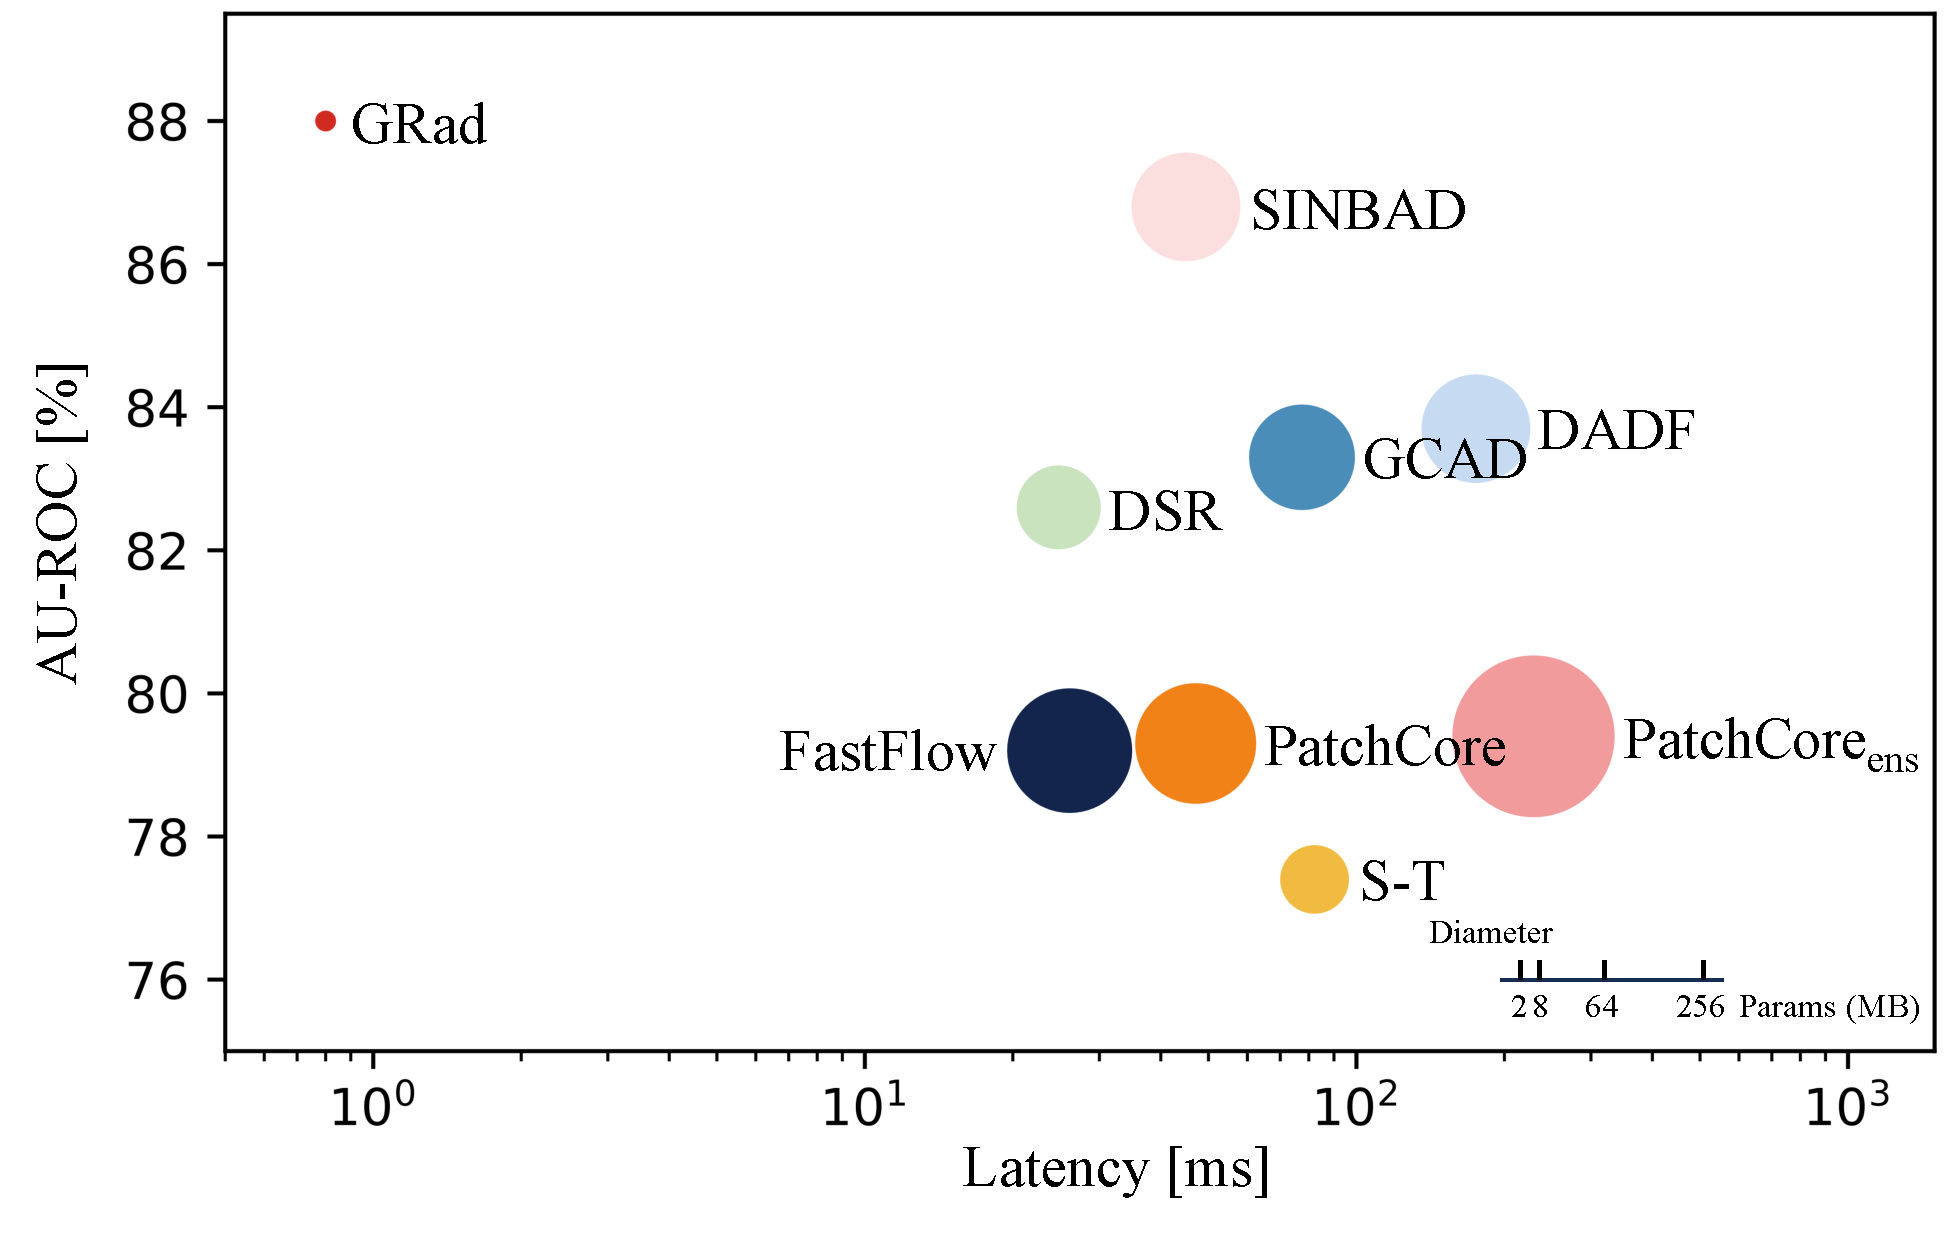
\includegraphics[width=1\linewidth]{images/speed.pdf}
    %removedVspace
    \caption{Anomaly detection performance vs. latency per image on an NVIDIA Tesla V100 GPU. Each bubble’s area is proportional to the number of parameters in each detector, and each AU-ROC value is an average of the image-level detection AU-ROC values on MVTec LOCO~\cite{MVloco}.}
    \label{fig: speed}
    %removedVspace
\end{figure}

Image anomaly detection plays a crucial role in various fields, including industrial product defect detection, medical image lesion detection, security screening using X-ray images, and video surveillance~\cite{ComplentaryGAN, MVTecAD, app1, app2, GANomaly}. However, securing real-world anomalous data for training is typically challenging and scarce due to the inability to cover a sufficiently diverse range of potential anomaly patterns. %%%%%ToBeFixed
Consequently, the setting of one-class learning, which employs only normal samples for model training, has proven to be better suited for most industrial anomaly detection tasks~\cite{MVTecAD, MVloco}.
In recent years, many high-accuracy industrial anomaly detection methods heavily rely on ImageNet~\cite{ImageNet10} pretrained feature extractor. Nevertheless, such reliance may limit their generalization capabilities in scenarios~\cite{MVloco} where ImageNet pretrained features are insufficiently informative, or on other types of image-like data~\cite{mvtec3D, BackTo3dFeatures}. Additionally, some methods have achieved promising results on the MVTec AD~\cite{MVTecAD} without using pretrained feature extractors. These methods utilize manually-selected external out-of-distribution (OOD) datasets~\cite{FCDD} or carefully designed anomaly-simulated data to sample anomaly patterns~\cite{CutPaste, DRAEM, SLSG}. However, previous anomaly acquisition strategies can be considered as ad-hoc solutions that overly rely on priors or visual inspection of test images, such as in MVTec AD, where most anomalies are low-level structure anomalies (\eg, scratches, dents, and contaminations). Such reliance may cause these strategies to fail in detecting other types of anomalies, such as logical anomalies recently proposed in the MVTec LOCO~\cite{MVloco}. These logical anomalies are represented as violations of logical constraints in images, which not only challenges the ananomaly simulation-based methods but also the pretrained representations by auxiliary datasets. Therefore, it becomes necessary to devise image anomaly detection techniques that are independent of both pretrained Imagenet feature extractors and ad-hoc anomaly acquisition strategies.

In this paper, we introduce a novel framework named \textbf{GRAD} (\textbf{G}enerating and \textbf{R}eweighting dense contrastive patterns for unsupervised \textbf{A}nomaly \textbf{D}etection), which achieves SOTA performance in both anomaly detection accuracy and inference runtime, as depicted in Fig.~\ref{fig: speed}. We first put forward a novel anomaly generation paradigm: retaining the structure information within each small patch of the image while disregarding the global structure information of the whole image. Based on this paradigm, we design an anomaly generator called PatchDiff. This generator enforces a constraint on the receptive field size of the diffusion model~\cite{DDPM} and removes the attention layers~\cite{AttentionNotNeed}, thus ensuring that only the local structure within each patch is retained, while the global structure is discarded. As illustrated in Fig.~\ref{fig: loco_generation_results}, with different sizes of the receptive field, PatchDiff can generate diverse dense contrastive patterns that cover a range of anomaly types, \eg, the structural and logical anomalies proposed in MVTec LOCO. Subsequently, we expect to utilize the generated local anomaly patterns to learn a patch-level anomaly detector. However, the contrastive patterns generated by PatchDiff may also be normal and we cannot provide patch-wise ground truth for them. Consequently, the generated contrastive patterns are unlabeled. Furthermore, the local patterns in both normal and generated data could often be long-tailed. Considering the previous two points, we introduce a self-supervised reweighting mechanism to mitigate the negative impacts of fake anomalous patches (patches without effective anomaly patterns) and imbalanced distribution. The mechanism utilizes density information of the features extracted by the detector during the training phase to assign different weights to the contrastive patches. It filters the fake anomalous patches and rebalances the distribution of the contrastive patches. Finally, to obtain high-throughput anomaly detection models better applied in practical industrial scenarios, we design a lightweight Fully Convolutional Network (FCN)-based patch-level detector with a pure encoder architecture. It consists of only 8 convolutional layers but performs on par with larger models in industrial anomaly detection. Furthermore, to deal with tasks that involve mixed-level anomalies, we can also integrate multiple detectors with different receptive fields. We empirically find that a single-level detector is enough to achieve competitive accuracy on MVTec AD dataset, while three detectors can be integrated to handle both structural and logical anomalies in MVTec LOCO.

\begin{figure}[!t]
    \centering
    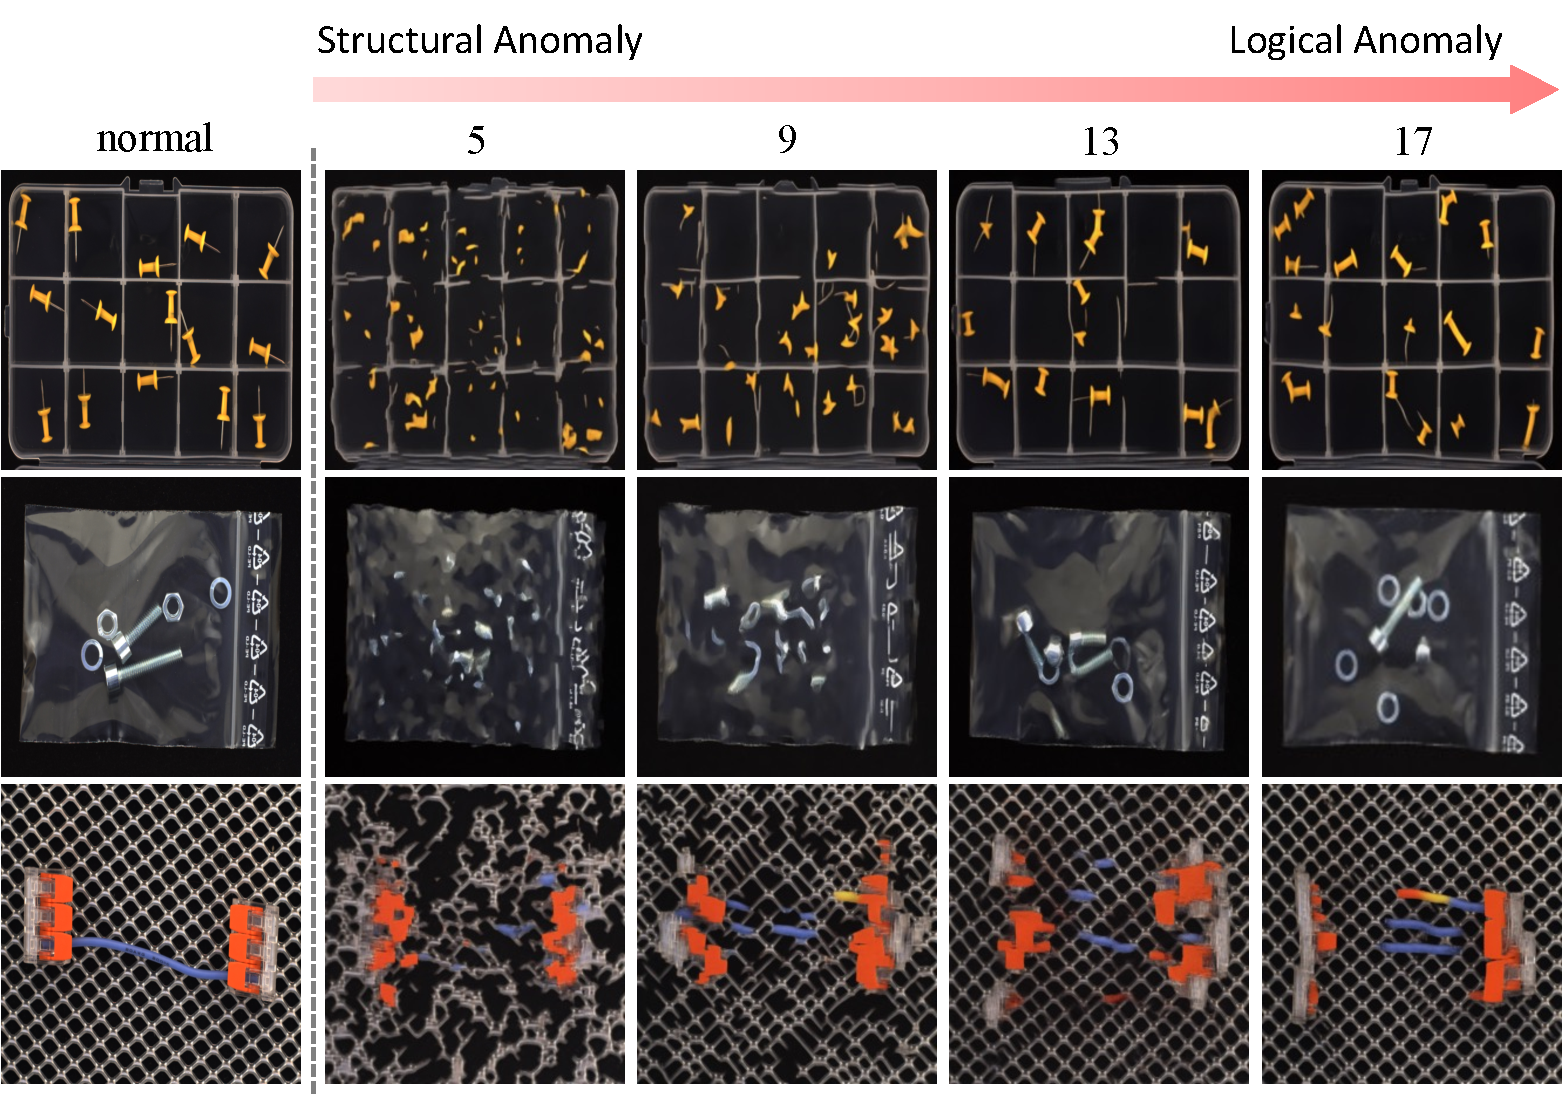
\includegraphics[width=\linewidth]{images/loco_generation_results.pdf}
    %removedVspace
    \caption{Anomaly contrastive images generated by our PatchDiff on MVTec LOCO. The number $n$ above the images indicates that this column is generated based on the corresponding $n \times n$ receptive field size. We show that employing varying sizes of limited receptive fields effectively enables the PatchDiff to expose anomalies at different levels: generators with smaller sizes tend to expose structural anomalies, while generators with larger sizes tend to expose logical anomalies.}%They provide dense contrastive patterns about how the normal images are combined by the elements at each level.
    \label{fig: loco_generation_results}
    %removedVspace
\end{figure}

The main contributions of this paper can be summarized as follows:
\begin{itemize}
    \item We propose a novel paradigm for generating anomaly patterns without scenario-specific priors. Based on this, we develop PatchDiff which can effectively expose a range of local anomaly patterns.
    \item We introduce a self-supervised reweighting mechanism for the generated contrastive data to rebalance them and filter out the fake anomalous patches. This mechanism enables we can efficiently use the unlabeled and long-tailed contrastive patterns for anomaly detection.
    \item We design a lightweight encoder-based patch-level detector trained with only the normal data and generated contrastive data, which relies on no external dataset, heavy pretrained backbone, or memory-consuming decoder architecture.
\end{itemize}


\section{Related Works}


\begin{figure*}[!t]
\centering
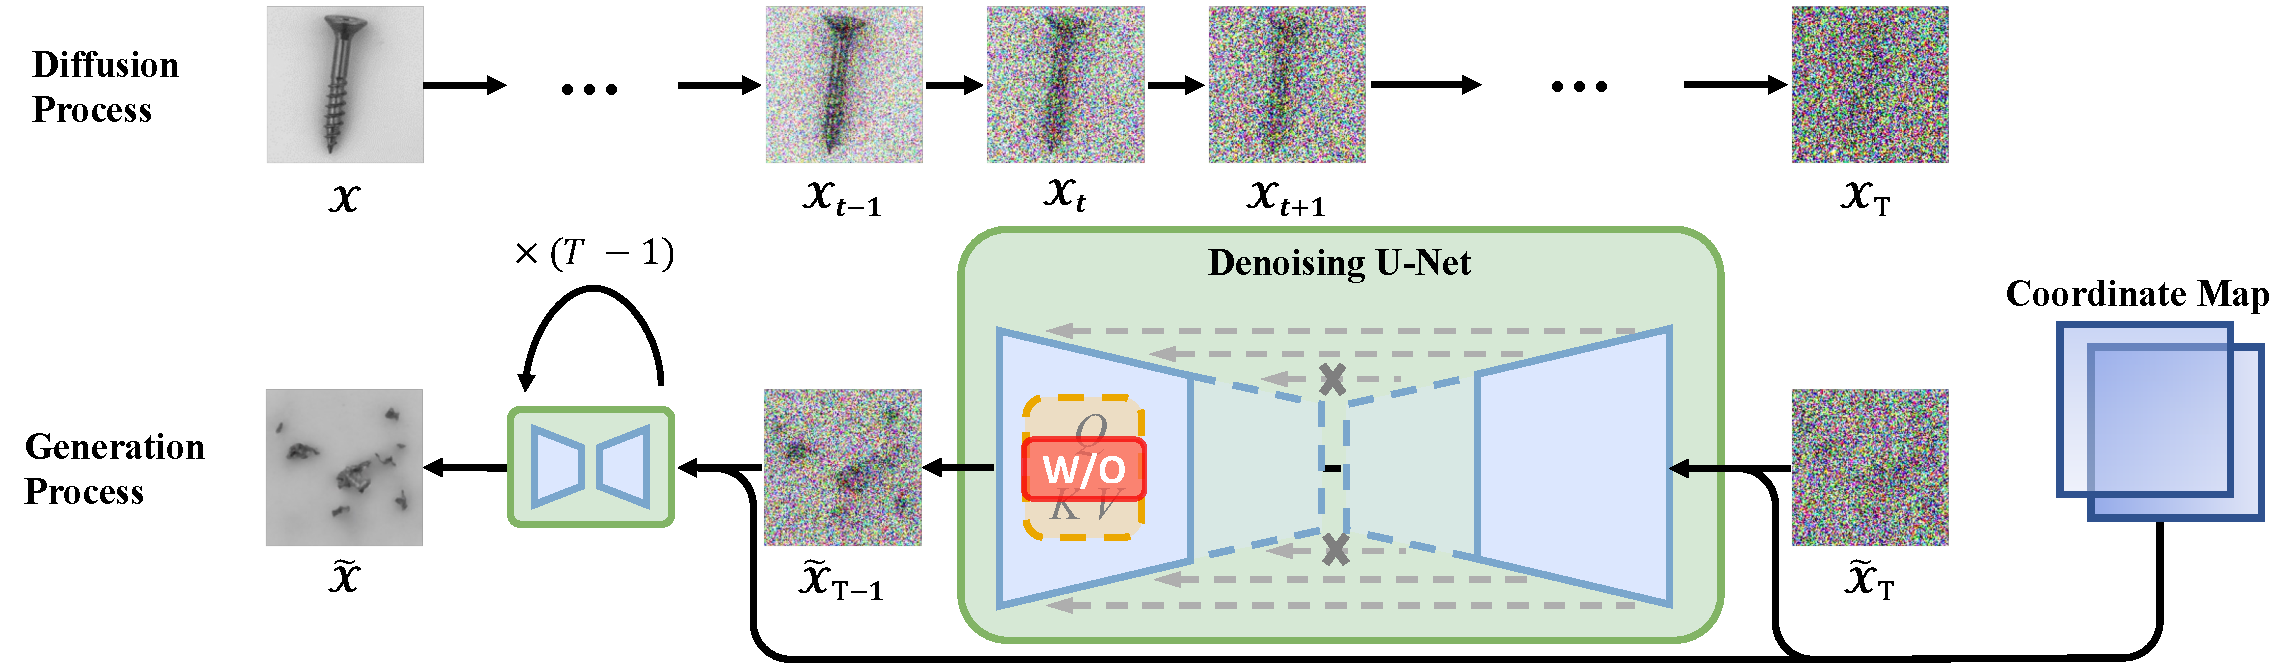
\includegraphics[width=\linewidth]{images/diffusion.pdf}
    \caption{An illustration of the proposed anomaly generator, PatchDiff. Compared with usual Diffusion models, PatchDiff limits the receptive field of the U-Net used to denoise, which preserves only the local structures rather than the global structures. PatchDiff can effectively produce higher-level novel visual structures coming from the recombinations of specific-level local structures. We can use PatchDiffs with various receptive filed sizes to generate multilevel dense contrastive patterns, which are useful for exposing the multilevel anomalies like the structure anomaly and the logical anomaly in MVTec LOCO.}
    \label{fig: PatchDiff}
\end{figure*}

\noindent\textbf{Reconstruction-based.}
A well-trained autoencoder (AE) on normal data is supposed to produce lower reconstruction errors on the normal data than the anomalous data~\cite{AE1, AE2, VAE}. However, in practice, it may also reconstruct anomalies very well or even better~\cite{Pidhorskyi2018GenerativePN}. To alleviate this problem, recent works developed many advanced variants of AE by using generative priors or novel architectures~\cite{OCGAN, MemAE, DAAD, RIAD, InTra, SSPCAB, UniAD}.

\noindent\textbf{Pretrained feature-based.}
State-of-the-art methods for industrial anomaly detection tend to use features of a deep network pretrained on external datasets (\eg, ImageNet). These methods~\cite{PaDiM, DifferNet, Cflow-ad, PatchCore, hyun2023reconpatch, zhang2023prototypical} effectively utilize the general low-level visual features encoded by the pretrained network to do the anomaly detection and achieve appealing performance on MVTec AD~\cite{MVTecAD}. However, they are hard to directly apply in other image-like domains (e.g. the depth map)~\cite{mvtec3D, BackTo3dFeatures} or to cover the higher-level anomaly type, logical anomalies~\cite{MVloco}.

\noindent\textbf{Anomaly simulation-based.}
% In the pertinent field of OOD~\cite{baseline_ood}, prior studies~\cite{Relu, OE, energyOOD} advocate for the utilization of outliers exposure to engender low confidence in the OOD space.
To overcome the limitations of pre-trained features and ensure that the model produces well-defined and expected results outside the normal distribution, several anomaly simulation methods~\cite{FCDD, CutPaste, DRAEM, SLSG} are proposed. They employ various ad-hoc strategies to simulate specific types of anomaly patterns tailored to different datasets. Most of them heavily rely on human priors and can only expose specific anomaly patterns, making them also challenging to generalize to different scenarios.
%In particular, our work is similar to the anomaly simulation-based methods but actually is generation-based.


\section{Approaches}

Our method can be primarily divided into two stages: (1) Generating diverse contrastive images based on our novel proposed anomaly generation paradigm to cover the anomaly patterns at interest levels. (2) Training lightweight patch-level detectors with our proposed reweighting mechanism to fully utilize the unlabeled and long-tailed generated contrastive patterns. In the following, we will describe the key parts of GRAD in detail.

\subsection{Generating anomaly Contrastive Images}
\label{sec: generating}

In contrast to previous ad-hoc anomaly acquisition strategies~\cite{CutPaste, DRAEM, SLSG}, we introduce a novel and prior-less anomaly generation paradigm: preserving the structure information within each small image patch while disregarding the global structure information of the entire image. To implement this, we propose a diffusion model~\cite{DDPM} based generator called PatchDiff.
As shown in Fig.~\ref{fig: PatchDiff}, the diffusion and denoise process is very similar to DDPM, the differences mainly come from the U-Net architecture in the following aspects:

(1) To prevent the U-Net from utilizing long-range information for recovering global structures during denoising, we deliberately remove self-attention used in DDPM~\cite{DDPM}. Self-attention is a powerful tool for capturing long-range contextual information, but for our specific task, it is unnecessary~\cite{AttentionNotNeed}, since local consistency is all we need.

(2) To further ensure that the U-Net focuses on recovering the local patterns within the corresponding patches during denoising, we directly reduce the depth of both the encoder and decoder of the U-Net. In this way, each latent neuron of the bottleneck has a limited receptive field, and thus it denoises using only the local content and retaining only local structures. %cover the patterns of each patch of corresponding size.

(3) To enable the U-Net to effectively model position-dependent cues, we incorporate a 2-channel coordinate map as additional information alongside the input. This coordinate map is a tensor with dimensions matching that of the input image, where each element represents the coordinate of the corresponding pixel. Noteworthy, the output of our U-Net is still a 3-channel image as same as the original U-Net in DDPM.

Then we modify the training loss of original Diffusion models by introducing a global tiny noise $\bepsilon_{g}$ during the noise injection process. It is motivated by the observation that there is a tendency for overall color deviation in the generated results. Consequently, to avoid the color deviation, the training loss of PatchDiff at each denoising step $t$ becomes
\begin{equation*}
\begin{aligned}
\mathbb{E}_{\bepsilon_1, \bepsilon_g}
\big\| \bepsilon_1 - \bepsilon_\theta\bigl(\sqrt{\bar{\alpha}_t} \mathbf{x}_0 + \sqrt{1-\bar{\alpha}_t} \bepsilon_1 + \bepsilon_g, t\bigr) \big\|^2,
\end{aligned}
\end{equation*}
where $\epsilon_{1}\sim\mathcal{N}(\mathbf{0}, \mathbf{I})$, $\epsilon_{\theta}$ and $\bar{\alpha}_t$ are the same as in DDPM.
% $\epsilon_{g}\sim\mathcal{N}(\mathbf{0}, \mathbf{I})$,
As depicted in Fig.~\ref{fig: loco_generation_results}, the images generated by PatchDiff effectively avoid the presence of low-level anomalous cues that often occur in simulation strategies, easily noticeable edges when tailoring two images together.
Instead, PatchDiff focuses more on the slightly higher-level anomaly patterns. By setting multiple receptive filed sizes to the U-Net, PatchDiff can efficiently expose both structural and logical anomalies in MVTec LOCO. This enables PatchDiff to produce more comprehensive local abnormalities without using any prior knowledge of test anomalies. Additionally, the reduction in the depth of architecture and the removal of attention layers contribute to a decrease in the model's complexity and calculation cost, leading to improved training and sampling speed. Furthermore, it is worth noting that the training process of PatchDiff uses only fitting loss like DDPM\cite{DDPM}, which is very stable and easy to implement. In summary, PatchDiff is a prior-less, easy-to-implemented, relatively-fast multilevel local anomaly pattern generation method.

\begin{figure}[!t]
\centering
    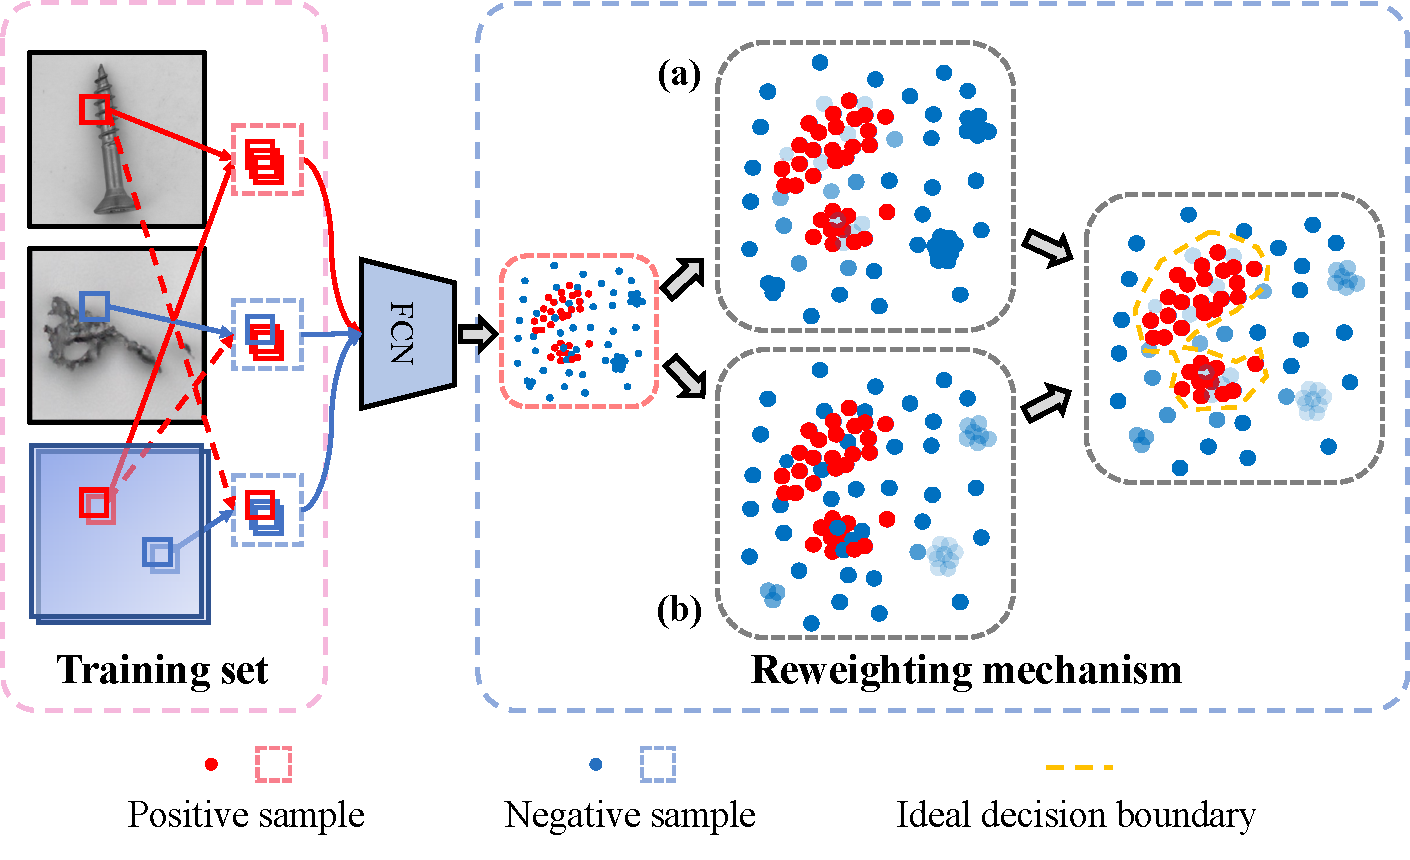
\includegraphics[width=1\linewidth]{images/training_detector.pdf}
    %removedVspace
    \caption{Schematic overview of two components during training patch-level detectors. The left portion is the training set which consists of one type of positive patch and two types of negative patches. The right portion is the reweighting mechanism which comprises mechanism (a) to filter the fake anomaly patterns and mechanism (b) to rebalance the long-tailed training data.}
    \label{fig: detector}
    %removedVspace
\end{figure}

\subsection{Training Patch-level Detector}
\label{sec: training}
A naive idea to utilize the contrastive images generated by PatchDiff is directly labeling them as the anomalous class and training image-level detectors. But it does not fully exploit the dense and local anomaly patterns nor provide useful anomaly scores for localization. Instead, we opt to train patch-level anomaly detectors that detect level-specific local anomalies by patch-wisely classifying the normal images and contrastive images.
Our patch-level detector is implemented with an 8-layer Fully Convolutional Network, FCN~\cite{FCN}, in a pure encoder way. At the training stage, the detector takes input patches of a fixed size, precisely $34 \times 34$ pixels, and produces an output anomaly score corresponding to each individual patch. To address local anomalies of multiple concerned levels (\eg, both structural and logical anomalies in MVTec LOCO), we choose to maintain the detector architecture but resize the original images into lower resolutions, which indirectly achieves the adjustment of the receptive field sizes. This approach enables us to train additional detectors capable of capturing higher-level anomaly patterns without redesigning the detector's architecture and further reduces the computational cost. In the following, we will introduce how to train the patch-level detector.
% We believe that reducing the resolution will not significantly affect the detection performance for higher-level anomaly patterns.
% To better elucidate the details of training the detector, in the following sections, we will introduce: 1) How to prepare the training set for detector training. 2) How to reweight the unlabeled and long-tailed contrastive patterns generated by PatchDiff. 3) How to further improve the detector's performance by regularization techniques.

\begin{figure}[!t]
    \centering
    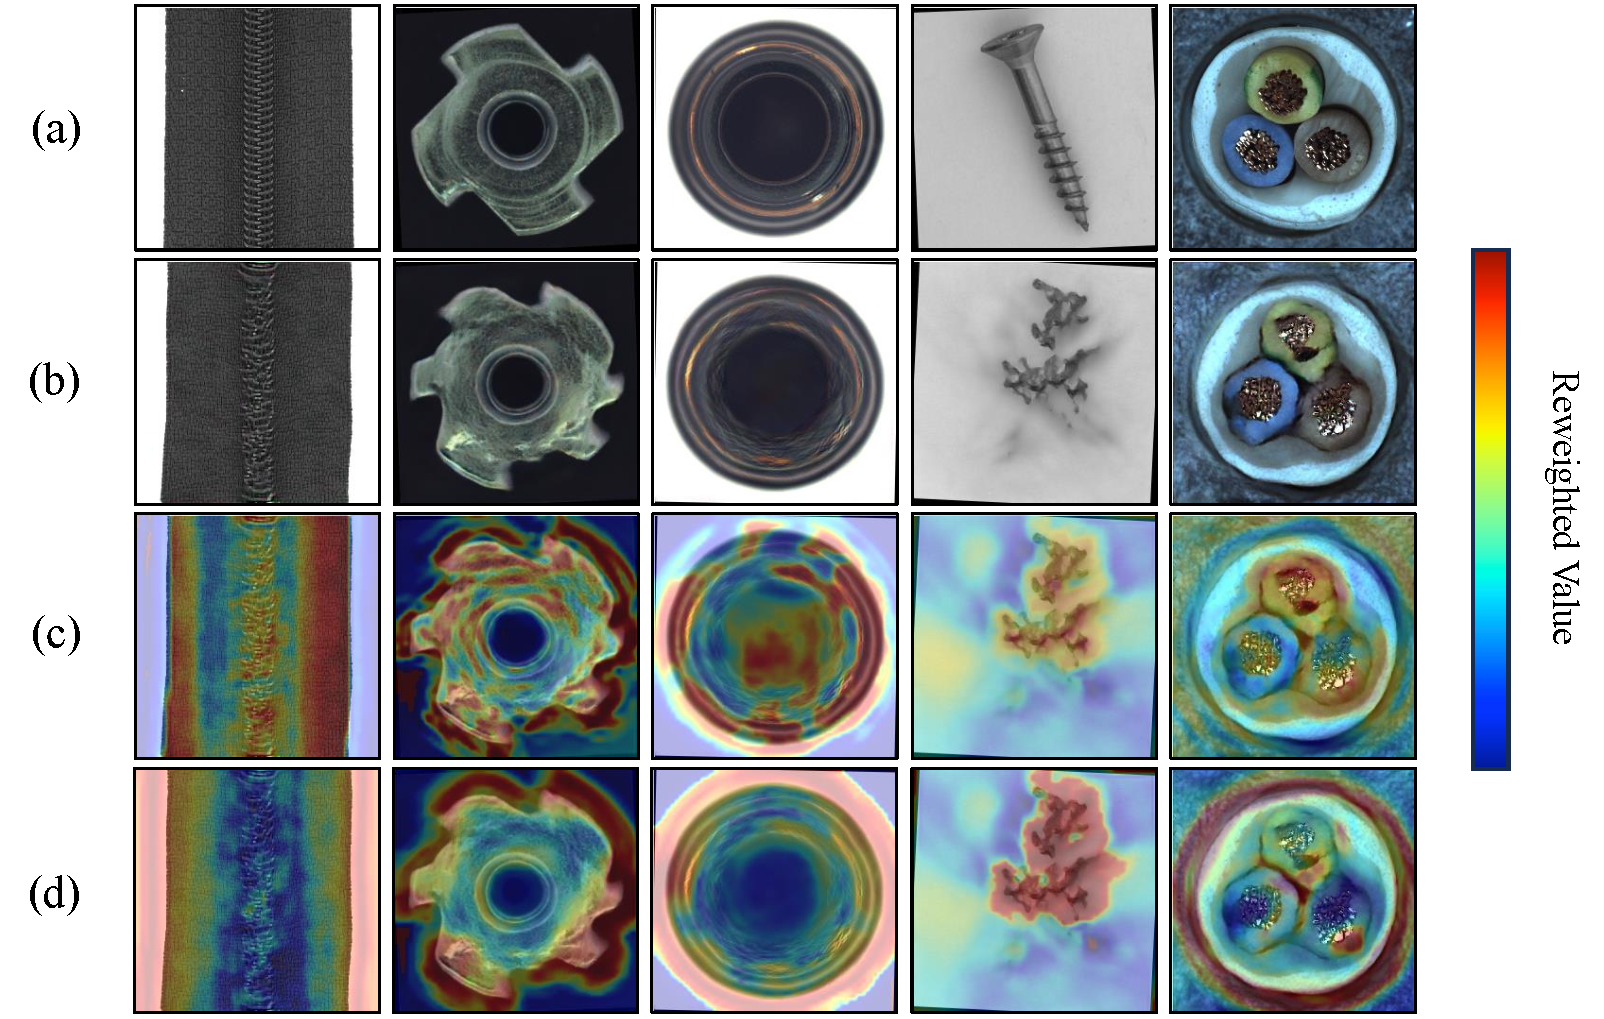
\includegraphics[width=1\linewidth]{images/reweighted_map.pdf}
    \caption{The reweighted map to show the effects of reweighting mechanism. (a) and (b) respectively displays the origin images and the generated contrastive images. (c) and (d) respectively depicts the effects when filtering fake anomaly patterns and rebalancing long-tailed training data. Our reweighting mechanism learns to identify patterns to be disregarded, indicated by the blue regions, and patterns to be emphasized, represented by the red regions, through a self-supervised approach} % Intuitively, at the training begins, the weights of patches are assigned with similar weights.
    \label{fig:reweightmap}
\end{figure}

\subsubsection{Preparing the Training set}

Similar to the input during the generation phase, we use a 2-channel coordinate map $F$ as an additional input. As illustrated in the left portion of Fig.~\ref{fig: detector}, we prepare three types of 5-channel patches as training inputs, including one type of positive patch and two types of negative patches. Let $I$ denote an image data, and $\mathcal{I}^{+}$ and $\mathcal{I}^{-}$ represent sets of normal samples and generated samples from PatchDiff, respectively. Subsequently, the positive patches set $\mathcal{C}^{+}$ and negative patches set $\mathcal{C}^{-}$ are defined as
\begin{equation*}
    \begin{aligned}
    \mathcal{C}^{+}=&\left\{c \mid c=\operatorname{RandCrop}(I\oplus F), I \in \mathcal{I}^{+}\right\},\\
    \mathcal{C}^{-}=&\left\{c \mid c=\operatorname{RandCrop}(I)\oplus \operatorname{RandCrop}(F), I \in \mathcal{I}^{+}\right\} \\
    &\cup\left\{c \mid c=\operatorname{RandCrop}(I\oplus F), I \in \mathcal{I}^{-}\right\},
    \end{aligned}
\end{equation*}
where $\oplus$ denotes concatenation along the channel axis. The negative patches are constructed in two ways: (1) the patches from generated samples along with their corresponding coordinate maps, and (2) the patches from normal samples with incorrect coordinate maps. Specifically, the patches from the latter way are believed to provide examples that break the dependence between patch content and position. This explicitly enhances the detector's utilization of the auxiliary information from the coordinate maps and improves its ability to capture position-aware cues.

\subsubsection{Reweighting the Contrastive Patches}
There are two potential challenges during training the patch-level detector $D$: (1) The images generated by PatchDiff are pixel-unlabeled, leading to the presence of fake anomaly patterns (e.g. the background region in the generated images) among the negative patches, which will mislead the detector. (2) Some important anomaly patterns may appear more rarely and lie in the low-density regions of the data manifold, causing the detector to overlook such patterns during the training process. To mitigate these challenges, we propose a feature density-based reweighting mechanism that incorporates two reweighting strategies, as shown in the right part of Fig.~\ref{fig: detector}. This mechanism relies on the feature distributions extracted from the last latent layer of our patch-level detector on both positive and negative samples. Let us denote $\mathcal{M}^+$ and $\mathcal{M}^-$ as the feature sets of positive and negative samples, respectively. Then the two reweighting strategies can be performed as follows:

(1) Filtering the fake anomaly patterns. As depicted in Fig.~\ref{fig: detector}(a), we introduce a reweighting factor $w^\text{noisy-}_i$ for each given negative patch $\bm{c}^-_i$, to assign smaller weights to the patches whose features are too close to or even within normal features set $\mathcal{M}^+$. The reweighting factor can be formulated as
\begin{equation}
    w^\text{noisy-}_i = \frac{1}{\sum_{\bm{z}\in\mathcal{M}^+} \exp(\beta_\text{density} \text{sim}(\bm{z},\bm{z}^-_i))} ,
\end{equation}
where $\bm{z}^-_i$ is the feature vector of the negative patch $\bm{c}^-_i$, $\mathrm{sim}(\bm{z}, \bm{z}'):= \bm{z} \cdot \bm{z}'/\lVert{\bm{z}}\rVert\lVert{\bm{z}'}\rVert$ is the density kernel based on the cosine similarity and $\beta_\text{density}>0$ is a hyper-parameter for controlling kernel bandwidth.

(2) Rebalancing the long-tailed training patches. As depicted in Fig.~\ref{fig: detector}(b), we introduce a reweighting factor $w^\text{tail-}_i$ for each given negative patch $\bm{c}^-_i$ to downweight the patches whose features are in the high-density regions. Empirically, we find introducing a reweighting factor $w^\text{tail+}_j$ for each positive patch $\bm{c}^+_j$ is also helpful. Therefore we have the following two additional reweighting factors for the training patches
\begin{equation}
\begin{aligned}
    w^\text{tail-}_i = \frac{1}{\sum_{\bm{z}\in\mathcal{M}^-} \exp(\beta_\text{density} \text{sim}(\bm{z},\bm{z}^-_i))},\\
    w^\text{tail+}_j = \frac{1}{\sum_{\bm{z}\in\mathcal{M}^+} \exp(\beta_\text{density} \text{sim}(\bm{z},\bm{z}^+_j))}.
\end{aligned}
\end{equation}

The effects of our reweighting mechanism are shown in Fig~\ref{fig:reweightmap}. By incorporating these two kinds of reweighting factors, our reweighted binary classification loss $\mathcal{L}_{\mathrm{RBCE}}$ can be formulated as
\begin{equation}
\label{eq: loss_function_rbce}
\begin{aligned}
    \mathcal{L}_{\mathrm{RBCE}}&=-\frac{1}{\lambda^+}\sum_{j=1}^{|\mathcal{C}^+|} w^\text{tail+}_j\log (1-f(\bm{c}^+_j))\\
    &\quad -\frac{1}{\lambda^-}\sum_{i=1}^{|\mathcal{C}^-|} w^\text{tail-}_i w^\text{noisy-}_i \log(f(\bm{c}^-_i)),
\end{aligned}
\end{equation}
where $\lambda^+$ and $\lambda^-$ are the normalization constants to keep the total weights of each class equal to 1:
\begin{equation}
\label{eq: regularization parameter}
    \lambda^+ = \sum_{j=1}^{|\mathcal{C}^+|} w^\text{tail+}_j,\quad
    \lambda^- = \sum_{i=1}^{|\mathcal{C}^-|} w^\text{tail-}_i w^\text{noisy-}_i.
\end{equation}
In practice, the $\mathcal{M}^+$ and $\mathcal{M}^-$ are both implemented with a memory bank that store the features of previous training steps in a queue.

\subsubsection{Regularization on Features and Gradients}
We further utilize a classical unsupervised representation learning method named denoising autoencoder ~\cite{DAE} to regularize the learned feature by detector $D$. To achieve that, we introduce a simple MLP-based network $R$ that recovers the original input patches from the feature vectors extracted from the last latent layer of $D$. Let $f_{Z}$ denote the function extracting features from input patches, $f_{R}$ denote the function recovering input patches from features, and $\mathcal{C}$ denote the collection of all training patches $\mathcal{C}^+\!\cup\!\mathcal{C}^-$. The feature regularization loss can be formulated as
\begin{equation}
    \begin{aligned}
	    \mathcal{L}_{\mathrm{feat}}= \frac{1}{|\mathcal{C}|}\sum_{\bm{c}\in \mathcal{C}} \left\|f_{R}(f_{Z}(\bm{c}+\bm{\epsilon_c})+\bm{\epsilon_z}) - \bm{c}\right\|^2,
     \end{aligned}
\end{equation}
where $\bm{\epsilon_c}$ and $\bm{\epsilon_z}$ are respectively the noise perturbations added to the feature layer and the input layer. The auxiliary denoising task regularizes the last hidden layer of the detector to extract informative and robust representations. We highlight the auxiliary network $R$ will be dropped in the inference stage so that will not increase the inference runtime.

Additionally, we propose a gradient regularization loss to smooth the learned decision function $f$, which further discourages the detector from learning imperceptible distinctions between normal patterns and fake anomaly patterns. The gradient regularization loss can be formulated as
\begin{equation}
    \mathcal{L}_{\mathrm{grad}}=\frac{1}{|\mathcal{C}^+|}\sum_{\bm{c}\in \mathcal{C}^+} \left\|\nabla_{\bm{c}} f(\bm{c})\right\|^{2}.
    \label{eq_gp}
\end{equation}
It penalizes the gradient norms of the decision scores with respect to the input data, which is often used to improve the Lipschitz smoothness and robustness, and thus the generalization performance of decision functions~\cite{GradPU, arjovsky2017towards,inputGrad}.
\subsubsection{The Overall Training Loss}

We calculate the overall training loss for the patch-level anomaly detector by aggregating the aforementioned three types of losses as
\begin{equation}
    \mathcal{L}=\mathcal{L}_{\mathrm{RBCE}} + \alpha_1 \mathcal{L}_{\mathrm{feat}} +\alpha_2 \mathcal{L}_{\mathrm{grad}},
\label{eq:final_loss}
\end{equation}
where $\alpha_1$ and $\alpha_2$ are hyper-parameters to adjust the impact of $\mathcal{L}_{\mathrm{feat}}$ and $\mathcal{L}_{\mathrm{grad}}$.

\begin{table*}[!ht]
\centering
    \label{tab:mvtec_main}
    \resizebox{0.95\textwidth}{!}{
    \begin{tabular}{c|c|c|c|c|c|c|c|c}
    \toprule
    Category & \makecell[c]{SPADE\\\tiny{\citealp{SPADE}}} & \makecell[c]{PaDiM\\\tiny{\citealp{PaDiM}}} & \makecell[c]{S-T\\\tiny{\citealp{S-T}}} & \makecell[c]{PatchCore\\\tiny{\citealp{PatchCore}}} &\makecell[c]{GCAD\\\tiny{\citealp{MVloco}}} & \makecell[c]{DADF\\\tiny{\citealp{DADF}}} & \makecell[c]{SINBAD\\\tiny{\citealp{SINBAD}}} & \makecell[c]{GRAD\\\tiny{Ours}} \\
    \midrule
    breakfast box
    & 78.2 & 65.7 & 68.6 & 81.3 & 83.9 & 75.3 & \textbf{92.0} & 81.2 \\
    juice bottle
    & 88.3 & 88.9 & 91.0 & 95.6 & \textbf{99.4} & 98.6 & 94.9 & 97.6 \\
    pushpins
    & 59.3 & 61.2 & 74.9 & 72.3 & 86.2 & 81.0 & 78.8 & \textbf{99.7} \\
    screw bag
    & 53.2 & 60.9 & 71.2 & 64.9 & 63.2 & 77.3 & \textbf{85.4} & 76.6 \\
    splicing connectors
    & 65.4 & 67.8 & 81.1 & 82.4 & 83.9 & 86.4 & \textbf{92.0} & 85.4 \\
    \midrule
    average
    & 68.8 & 68.9 & 77.3 & 79.3 & 83.3 & 83.7 & 86.8 & \textbf{87.5} \\
    \bottomrule
\end{tabular}}
\caption{Image-level AU-ROC performance for anomaly detection of different methods on MVTec LOCO~\cite{MVloco}. The best results are in bold.}
\label{tab: auc_mvtec_loco}
\end{table*}

\begin{figure*}[!htbp]
\setlength{\belowcaptionskip}{0.0cm}
\setlength{\abovecaptionskip}{0.1cm}
    \centering
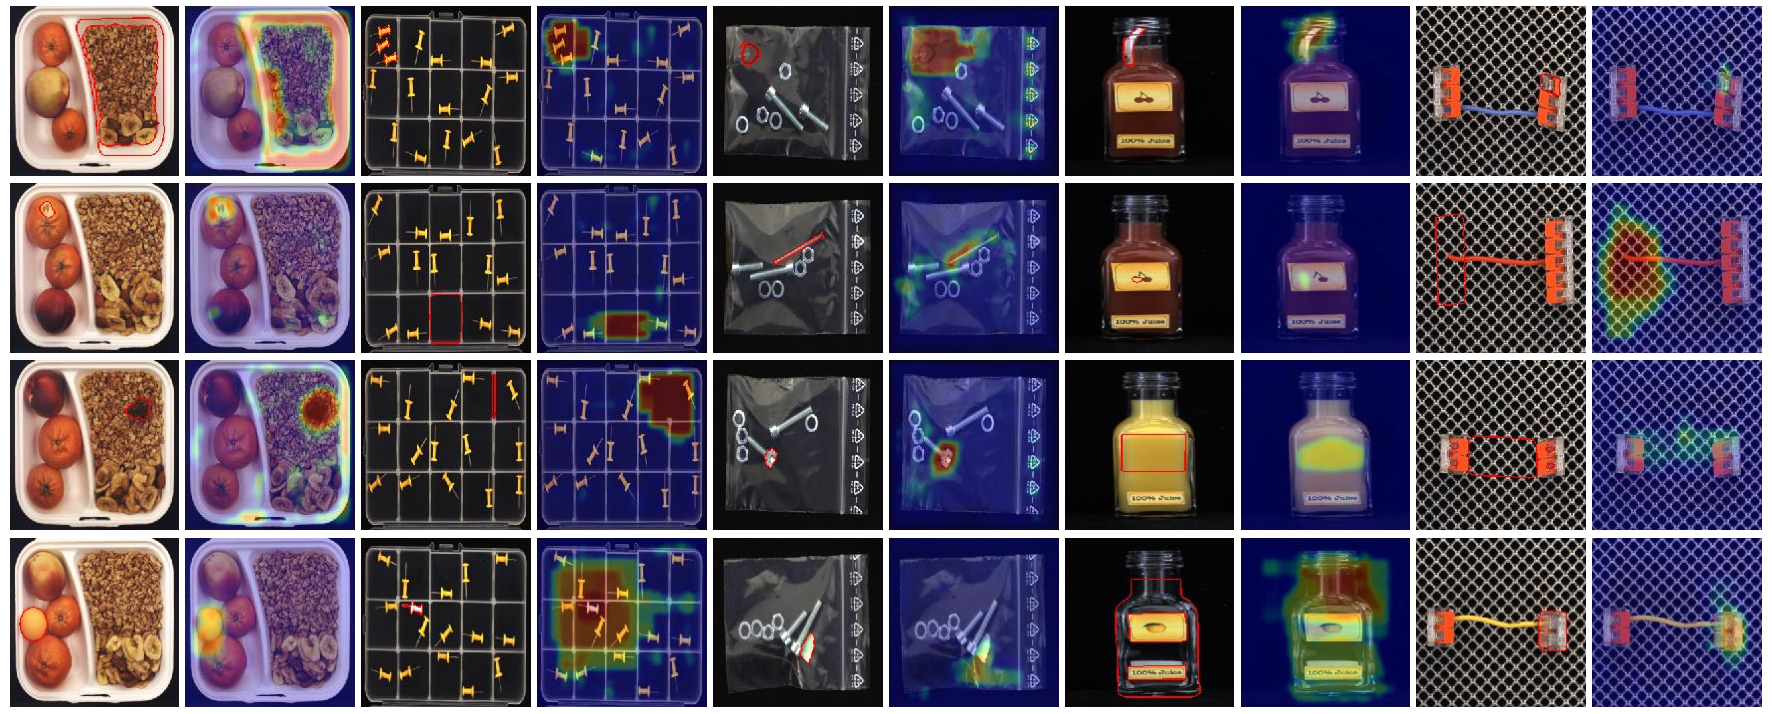
\includegraphics[width=0.9\linewidth]{images/loco_results.pdf}
    \caption{Defect localization results of GRAD on MVTec LOCO~\cite{MVloco}. } %on cable, hazelnut, metal nut, screw, grid, carpet The last column shows the failure cases. More examples can be found in Appendix.
    \label{fig: main_results}
\end{figure*}

\section{Experiments}

In this section, we first briefly introduce the experimental details (See Appendix for more details). Then we report the anomaly detection accuracies and the ablation study on each component. % Finally, we show the failure cases of GRAD.

\subsection{Dataset}

To validate the effectiveness and generalizability of our approach, we perform experiments on both MVTec AD~\cite{MVTecAD} and MVTec LOCO~\cite{MVloco}. There are 15 sub-datasets in MVTec AD and 5 sub-datasets in MVTec LOCO and each sub-dataset presents a diverse set of anomalies.
% Both of them contain high-resolution industry images of multiple categories. The images are collected in realistic scenes and cover both aligned and unaligned objects.
Particularly, the training sets among them contain only normal images, while the test sets contain both normal and various types of industrial defects. Pixel-level annotations are provided in the test set.

\subsection{Training Settings}

We simply define level-$n$ PatchDiff as the PatchDiff with a receptive field of $n \times n$ pixels, and the images generated by it belong to level-$n$. Similarly, we define level-$n$ detector as the patch-level detector with an indirect receptive field of $n \times n$ pixels.

\noindent\textbf{PatchDiff}. For each sub-dataset in MVTec AD, we train 3 levels of PatchDiffs (level-5, 9, 13). For each sub-dataset in MVTec LOCO, we need to train 3 different levels of detectors, and consequently, we train 4 levels of PatchDiffs (level-5, 9, 13, 17). In particular, 2 of them use level-5, 9, and 13 PatchDiffs and another one uses level-9, 13, and 17 PatchDiffs. For all PatchDiffs, we generally train them for a total of 10,000 training steps. For each sub-dataset, we sample 1,000 images for each level-$n$.

\noindent\textbf{Patch-level Detector}. Each sub-dataset in MVTec AD and MVTec LOCO contains limited training images. To train competitive detectors from scratch for each small sub-dataset, we adopt general data augmentations on both normal and generated images like previous works\cite{MVTecAD, MVloco}. For level-$34, 68,$ and $136$ detectors, the images are respectively resized into $256\times256$, $128\times128$, and $64\times64$. We train the detector on batches of size $128\times(k+2)$ for 2,000 epochs and report the accuracy of the final epoch. Each batch contains 128 randomly cropped positive patches from 4 normal images and $128\times(k+1)$ negative patches from 4 normal images and $4k$ contrastive images, where $k$ equals the number of levels of used generated contrastive images. Specifically, we use $k=3$ for all experiments as mentioned before.

\subsection{Evaluation Settings}
The image-level anomaly score directly takes the max value of a score map from the patch-based anomaly detector, and the pixel-level detection result is obtained by up-sampling the score map and then applying a Gaussian blur with a kernel size of 16. Consistent with existing methods~\cite{MVTecAD, MVloco}, we use AU-ROC as the evaluation metric for the evaluation of image-level anomaly detection and pixel-level anomaly localization.

\begin{table}[htbp]
% \footnotesize
\centering
\setlength{\belowcaptionskip}{0.0cm}
\setlength{\abovecaptionskip}{0.1cm}
\resizebox{0.9\linewidth}{!}{
% \setlength{\tabcolsep}{2pt}{
\begin{tabular}{lcc}
\toprule
Method & \makecell[c]{Pixel-level\\AU-ROC} & \makecell[c]{Image-level\\AU-ROC} \\
\midrule
IGD\tiny{~\citep{IGD}} & 93.1 & 93.4 \\
PSVDD\tiny{~\citep{PSVDD}} & 92.5 & 93.2 \\
FCDD\tiny{~\citep{FCDD}} & 92.1 & 95.7 \\
CutPaste\tiny{~\citep{CutPaste}} & 95.2 & 96.0 \\
NSA\tiny{~\citep{NSA}} & 96.3 & 97.2 \\
DRAEM\tiny{~\citep{DRAEM}} & \textbf{97.3} & 98.0 \\
DSR\tiny{~\citep{DSR}} & - & 98.2 \\
\rowcolor{gray!20} GRAD \tiny{(Ours)} & 96.8 & \textbf{98.7} \\
\bottomrule
\end{tabular}}
\caption{Anomaly detection performance on MVTec AD dataset~\cite{MVTecAD}. The best results are in bold.}
\label{tab: auc_mvtec}
\end{table}

\subsection{Main Results}

\noindent\textbf{The anomaly detection results.} We compare GRAD with different methods on MVTec AD and MVTec LOCO, as shown in Table~\ref{tab: auc_mvtec_loco} and Table~\ref{tab: auc_mvtec}. For both datasets, GAD has the best average image-level AU-ROC score, demonstrating the effectiveness of GRAD in anomaly detection. In table~\ref{tab: auc_mvtec_loco}, it is important to note that the fairness of the comparison might be compromised to some extent, as all the compared methods utilize ImageNet pretrained feature extractors. However, GRAD still achieves superior performance by 0.7\% even without such advantages, which shows that ImageNet pretrained features inadequately address the intricacies of logical anomaly detection within MVTec LOCO, and further demonstrates that our contrastive images generated by PatchDiff do expose both structural and logical anomalies effectively. In particular, GRAD achieves excellent results (+13.5\%) on the sub-dataset of pushpins, which exactly fits our observation that the generated images for pushpins perfectly expose several abnormal logical situations in the testing set, \eg, the additional pushpin in the top left compartment and no pushpins in the top right compartment, as shown in level-17 generated pushpin image of Fig.~\ref{fig: loco_generation_results}. In addition, we show the defect localization results in Fig.~\ref{fig: main_results}. In table~\ref{tab: auc_mvtec}, all the methods we compared do not rely on pretrained features and external data. Although GRAD does not achieve the best result for anomaly localization (pixel-level AUROC), it is still competitive among them.


\noindent\textbf{Inference runtimes.} We compare and report the inference latency and FPS in Table~\ref{tab:GRad_speed}. Obviously, GRAD achieves a remarkable throughput performance due to its extremely lightweight architecture, and thereby, GRAD's inference speed is more than 16 times faster than GCAD's.

\begin{table}[!htbp]
\centering
\setlength{\belowcaptionskip}{0.0cm}
\setlength{\abovecaptionskip}{0.1cm}
\resizebox{0.9\linewidth}{!}{
\begin{tabular}{lrr}
    \toprule
    Method & latency (ms$\downarrow$) & FPS$\uparrow$ \\
    \midrule
    S-T\tiny{~\cite{S-T}} & 82.2 & 12.2 \\
    FastFlow\tiny{~\cite{FastFlow}} & 26.1 & 38.3 \\
    DSR\tiny{~\cite{DSR}} & 24.8 &40.3 \\
    GCAD\tiny{~\cite{MVloco}} & 12.9 & 77.5 \\
    PatchCore\tiny{~\cite{PatchCore}} &47.1 &21.2 \\
    \rowcolor{gray!20} GRAD \tiny{(Ours)} & \textbf{0.799} & \textbf{1251.6}\\
    \bottomrule
\end{tabular}}
\caption{Inference speed on NVIDIA Tesla V100. The data of our method is obtained on MVTec LOCO dataset with three patch-level detectors (patch size: 34, input size: 256, 128, and 64).}
\label{tab:GRad_speed}
\end{table}

\begin{table}[!htbp]
\centering
\setlength{\belowcaptionskip}{0.0cm}
\setlength{\abovecaptionskip}{0.1cm}
\resizebox{\linewidth}{!}{
\begin{tabular}{lccc}
\toprule
& & \footnotesize{AUROC} & \\
% \cmidrule{2-4}
& Level-34 & Level-68 & Level-136 \\
\midrule
baseline\dag & 78.2 & 77.8 & 64.3\\
+ Regularization & 81.6 & 80.9 & 65.2\\
+ Noisy Reweighting & 82.5 & 82.5 & 72.1 \\
+ Long-tail Reweighting & 85.2 & 85.4 & 75.1\\
\bottomrule
\end{tabular}}
\caption{Ablation study on components. Detection AUROC results on MVTec LOCO dataset of three patch-level detectors are presented. \dag The baseline setting uses no regularization techniques and reweighting strategies.}
\label{tab: ablation_component}
\end{table}

% \begin{table}[!htbp]
% \centering
% \setlength{\belowcaptionskip}{0.0cm}
% \setlength{\abovecaptionskip}{0.1cm}
% % \begin{tabular}{ccc|c}
% % \toprule
% % \multicolumn{3}{c|}{Configurations}& Detection  \\
% % L136 & L68 & L34  & AUROC \\
% % \hline
% % \hline
% % \checkmark &   &    &  unkown   \\
% % & \checkmark &  & 85.4 \\
% % & & \checkmark & 85.2\\
% % \midrule
% % \checkmark & \checkmark &      &  unkown     \\ %
% % \checkmark &    & \checkmark   &  unkown \\
% %  & \checkmark & \checkmark  & unkown \\
% %  \midrule
% % \checkmark & \checkmark & \checkmark &  $\textbf{unkown}$  \\
% % \bottomrule
% % \end{tabular}
% \begin{tabular}{l|ccccccc}
% \toprule
% Level-136 & \checkmark & & & \checkmark & \checkmark & & \checkmark \\ %\cline{3-3} \cline{6-6} \cline{9-9}
% Level-68 & & \checkmark & & \checkmark & & \checkmark & \checkmark \\ %\cline{3-3} \cline{6-6} \cline{9-9}
% Level-34 & & & \checkmark & & \checkmark & \checkmark & \checkmark \\ %\cline{1-1} \cline{3-3} \cline{6-6} \cline{9-9}
%   \midrule
%   AUROC & - & 85.4 & 85.2 & - & - & - & 88.2\\ %\cline{9-9}
% \bottomrule
% \end{tabular}
% \caption{Ablation study about detector levels on MVTec LOCO dataset.}
% \label{tab: ablation_GRad_level}
% \end{table}

\subsection{Ablation study}

We first perform an extensive ablation study to validate the effectiveness of two reweighting factors and the regularization technique on MVTec LOCO. The results are shown in Table~\ref{tab: ablation_component}. More details and comprehensive ablation results can be found in Appendix. We utilize the baseline as the beginning and then add regularization, noisy reweighting and long-tail reweighting one by one.
% This allows us easily to report that the regularization techniques help detectors learn better representations and smooth decision boundaries, and further show that the fake anomaly patches and long-tail distribution do interfere with the performance of the detectors, and it is clear that our reweighting mechanism does effectively mitigate them from these two aspects.

\textbf{Effects of regularization techniques.} One of the novel contributions presented in this paper is the regularization on features and gradients, which helps our encoder-based detector extract an informative and robust representation and build a smooth decision boundary for the data manifold. As demonstrated in Table~\ref{tab: ablation_component}, the integration of these techniques translates into improvements of +3.4/+3.1/+0.9 on the MVTec LOCO dataset.

\textbf{The effect of reweighting mechanism.} Our reweighting mechanism comprises two essential components: (1) noisy reweighting, which aims to filter fake anomaly patches, and (2) long-tail reweighting, designed to rectify the imbalanced distribution of input data. When integrating the noisy reweighting, our detectors display enhancements of +0.9/+1.6/+6.9 on the MVTec LOCO dataset, as presented in Table~\ref{tab: ablation_component}. Furthermore, with the incorporation of long-tail reweighting, our detectors achieve improvements of +2.7/+2.9/+3.0, as shown in the same table. These outcomes underscore the disruptive influence of fake anomaly patches and the presence of long-tail distributions on detector performance. It is evident that our reweighting mechanism adeptly mitigates these challenges from both fronts, offering substantial advantages to our detectors.

Particularly, in Table~\ref{tab: ablation_component}, Level-136 detectors exhibit relatively poorer performance in anomaly detection. This result can be attributed to their input size, which is merely $64 \times 64$, resulting in insufficient resolution to offer informative structural anomaly details. However, this is in line with our intentions, as the purpose of Level-136 detectors is not to emphasize minute details, but rather to capture the logical relationships among components within the receptive fields of size $136 \times 136$.

% \subsection{Failure Cases}

% We show the failure cases at generation stage in Fig~\ref{fig:failure_case_generation} and the failure cases at detection stage in last coloums of Fig~\ref{fig:main_results}.

\section{Conclusion}
In this paper, we propose a novel unsupervised anomaly detection framework, GRAD, by generating and reweighting dense contrastive patterns. The proposed generation method PatchDiff is able to generate multilevel contrastive patterns which exposes a range of local anomaly patterns. The proposed reweighting strategies fully utilize the unlabeled and long-tailed contrastive patterns and help the patch-level anomaly detector better learn the exposed local anomaly patterns. GRAD requires no scenario-specific prior, external datasets, or heavy pretrained feature extractor. It achieves competitive anomaly detection and localization accuracy with a superior inference speed.

Further refinements to GRAD can be explored: 1) Advancing the algorithms for handling long-tailed and noisy labeled data, thereby utilizing the potential of the generated dense contrastive patterns more effectively. 2) Investigating the feasibility of integrating multiple patch-level detectors into a single lightweight network. 3) Exploring better network architecture and training settings for PatchDiff.

\section{Acknowledgements}

This work is supported in part by Shanghai science and technology committee under grant No. 21511100600.  We appreciate the High Performance Computing Center of Shanghai University, and Shanghai Engineering Research Center of Intelligent Computing System for providing the computing resources and technical support. Additionally, we extend our heartfelt appreciation to Professor Jincheng Jin and Weizhong Zhang from Fudan University, as well as Associate Professor Bin Li, for their invaluable assistance and insights during the writing process of this paper. Their expert guidance and stead- fast support were instrumental in the successful completion of this research.


Voluptatibus veniam est odit modi quas architecto suscipit, harum reprehenderit beatae recusandae consequuntur sunt saepe eveniet.Deleniti ad molestias non nobis quaerat dolorum, ipsam voluptate dolor neque ab deserunt esse, optio soluta maiores deleniti nulla ipsa cupiditate quod.Tenetur consequatur fugit ea ipsa voluptates sapiente mollitia maxime, nostrum sapiente ut non laborum minima accusamus, unde illum odio voluptate eligendi tempore amet, molestias magni dolor fuga atque veritatis consectetur totam commodi fugiat soluta.Perferendis libero optio quos dolorum mollitia, accusamus eaque excepturi cumque earum, dolores eum ipsam ipsa maxime ullam sit, error facilis sunt incidunt earum quasi eius ab?Quidem earum nesciunt dolore accusantium quia ut, eum dicta cupiditate consequatur quam eaque porro ea vero, porro tempore iste possimus labore?Sunt cupiditate obcaecati excepturi beatae quaerat, incidunt modi sit unde ad nostrum molestiae perferendis adipisci obcaecati veritatis, mollitia architecto non incidunt modi voluptatem ipsa, accusantium quae blanditiis eveniet commodi ipsa officia velit eum vel, iusto rem tenetur temporibus cupiditate deserunt impedit?Ex eius assumenda iste dicta, adipisci ut veritatis labore.Quam similique veritatis nobis illum voluptates ex nostrum quae doloremque placeat pariatur, quas libero nulla aliquid tenetur itaque ad, delectus vitae beatae doloremque debitis repellat dignissimos inventore, quis voluptatem id adipisci, quos officiis porro dolorum adipisci excepturi expedita reiciendis voluptas nobis maiores sit.Id eum placeat fuga facere illo dolore inventore maxime doloribus, assumenda animi sed quo ipsam doloribus temporibus aliquam nemo, esse provident cupiditate rerum eius, veniam corrupti quos aliquid saepe animi libero ratione omnis ipsa, beatae optio blanditiis dolores non aliquam earum suscipit eaque temporibus?Repudiandae repellat vitae cupiditate corrupti maiores quos nihil ullam, ullam rem dolorem impedit?Porro facere atque eveniet optio sunt, placeat magni ducimus exercitationem natus saepe itaque.Error quas sapiente a unde, eveniet consequuntur possimus sint assumenda inventore incidunt quis, consectetur molestias illum, perspiciatis sed explicabo?Deleniti modi est quia dicta illo ratione cupiditate laboriosam non, molestias magni accusamus est necessitatibus suscipit molestiae totam obcaecati natus ut a, ducimus repellendus quas, doloremque voluptatum velit ipsa minus omnis officia accusantium quaerat, mollitia et voluptatum repellendus magni deserunt iste.Perspiciatis nulla rerum corporis illo explicabo omnis officia dignissimos, nihil hic dolor distinctio officia ab, harum commodi veritatis aperiam odit eius ea vitae minus earum perferendis, minus ullam totam esse?Error dignissimos quas fuga itaque facere libero, neque alias aut impedit dolorem mollitia, corrupti nesciunt voluptate sed, assumenda velit alias enim deleniti minus voluptatum et perspiciatis repellendus recusandae tenetur, iste distinctio libero id aliquam velit quidem tempora voluptatibus molestiae voluptas?Rerum nemo neque beatae earum corporis porro amet autem, consequuntur tenetur totam ex iure illo?Voluptatem facilis porro quo quod exercitationem recusandae eaque assumenda, facere a asperiores eum at nam, architecto nam tempore.Iusto magni sit aut nam fuga perspiciatis sequi excepturi, repellendus deleniti voluptate voluptates laboriosam distinctio iste mollitia quasi unde atque architecto, debitis excepturi vel blanditiis neque vero voluptates iste optio nostrum?Magnam illo quos adipisci distinctio quaerat vitae minus voluptates reprehenderit commodi, necessitatibus minus officia doloribus in asperiores quam.Aperiam animi tempore ipsum quisquam, nihil quam fugiat recusandae placeat nesciunt cupiditate facere, voluptatum necessitatibus praesentium exercitationem libero fugiat reiciendis nobis laudantium natus maxime, expedita sed rem, iure est corporis in fuga sint cupiditate impedit ipsam recusandae et.Quae sapiente quas consectetur commodi quos expedita quasi, dolore asperiores eveniet autem possimus laboriosam vitae quisquam nihil, quia dolore voluptatibus adipisci consectetur non, at voluptates architecto.Beatae commodi quas facilis et blanditiis placeat eveniet nemo, consectetur blanditiis in atque est ipsam facere praesentium quam inventore numquam expedita, ad voluptatibus ab delectus neque deserunt aspernatur voluptatum sed distinctio odio omnis, facilis laborum explicabo asperiores eos quisquam ex a fugit assumenda cum, provident sed doloremque qui?Culpa quidem quaerat reiciendis nam adipisci cumque aut, provident ducimus asperiores iusto iste ipsum ullam facere ratione harum, error pariatur vero vel id, ab eaque reiciendis, impedit eum repellat ex fugiat veritatis voluptatum perferendis omnis illum.Assumenda fugit fuga sunt, doloribus excepturi repellat, nobis ea laborum blanditiis incidunt nihil culpa doloribus rem cumque rerum, exercitationem tenetur quos porro odio blanditiis consequuntur ipsa quasi consectetur itaque eveniet.Qui architecto dolorum voluptate excepturi, veritatis quas fugiat, deserunt fugiat ex, nesciunt unde esse nostrum odit ab tempore dolore, assumenda est accusamus laborum repudiandae fugiat ipsam totam nobis.Quis eligendi et molestiae libero quod assumenda optio, optio numquam cupiditate quam sapiente, reprehenderit illum nobis eaque natus deleniti dolorum autem quas?Accusantium molestiae tenetur inventore, libero esse iure qui beatae iusto quam cupiditate ducimus, asperiores eum vitae ipsam voluptas dolore natus est eos suscipit, minus fugit molestias?Ratione nam quae ducimus totam minima unde quis deserunt, enim ducimus omnis dolorem modi minus labore quo fuga id dolor, voluptatum architecto necessitatibus dolores fugit inventore consectetur reprehenderit?Placeat quia veritatis alias dolorum a sint id aperiam eligendi dolore, eligendi excepturi autem dolorem facere est, nesciunt minus qui expedita nisi reprehenderit maxime repudiandae sequi tenetur quis, dolor perferendis accusantium voluptas blanditiis illo.Asperiores quo excepturi incidunt laboriosam ab, itaque dignissimos a?Enim laboriosam nulla minus similique illum sequi, harum sunt sequi neque cumque, minima voluptatibus recusandae maxime praesentium, quaerat debitis commodi odit iure quo corrupti, eligendi nostrum totam quam repellendus animi fuga adipisci aspernatur dolor vero non?Sed quis praesentium sapiente at aspernatur officia velit saepe laudantium sunt esse, sed quia voluptate ut eaque perferendis exercitationem asperiores numquam, neque id aliquid eaque quasi reiciendis quisquam beatae a quod, odio fugiat facilis tempora minus dignissimos magni, consectetur dicta assumenda enim distinctio neque nulla repellat reprehenderit odit non consequatur?Ab maxime facere iure pariatur, libero odio sint totam fugiat sed inventore cumque, vero excepturi fugit odit, deserunt eius deleniti libero perferendis quae.Earum doloremque labore vitae excepturi ipsa optio ipsum facere quas blanditiis dolore, provident explicabo iusto tempore maiores animi laudantium dolorum quaerat quis similique.Non doloremque et nesciunt facilis adipisci commodi consectetur fuga voluptates totam quaerat, obcaecati molestiae iure, debitis rerum exercitationem dolorem error possimus inventore reprehenderit quis, adipisci ipsa ab, eligendi veritatis aliquid suscipit consequuntur voluptatem ab laudantium error accusamus cupiditate.Inventore tempore eum totam voluptatem unde expedita, non quaerat dolores aperiam quod?Vel perspiciatis est, voluptas atque quos velit inventore adipisci, harum esse repellat asperiores recusandae?Voluptas doloremque ab itaque optio rem delectus qui ex, dolores vel animi consequuntur rem ipsum, laboriosam tempora sint unde accusamus itaque vitae aut ea quam placeat fuga, voluptatibus quam expedita sed iure?Eaque veritatis non sint unde delectus autem quam alias, quaerat fuga ullam corrupti at nostrum delectus porro, error excepturi repellendus, dolor soluta tenetur?Perspiciatis error rem corporis, esse officiis voluptatem error officia nam fuga, amet voluptatem cum doloremque odit exercitationem cupiditate ab optio a, saepe nostrum aut fugiat ex delectus odit ipsa quasi enim ducimus?Nulla neque nisi non accusamus ipsam magni aut necessitatibus laborum, pariatur tempore quo molestias mollitia totam, voluptates debitis eligendi repudiandae accusamus modi iure recusandae laboriosam neque, distinctio vel doloremque veniam sapiente ab?Voluptatem corrupti dolorum voluptatum aperiam esse qui non ad quisquam aut suscipit, nostrum autem asperiores quibusdam ipsam animi eum nam quod, voluptatem atque quidem voluptas nisi ad mollitia magni quia saepe nihil eum, libero doloribus facere nisi quidem quos eveniet magni?Fugiat eius explicabo, minus accusantium sequi possimus ea eveniet veniam quas, vitae eos sed, nam eos molestiae natus ad nihil autem dolores consequatur?Tempore accusantium deleniti quidem corrupti aspernatur explicabo, corrupti beatae numquam magni excepturi, eaque similique ab, quos nisi odit distinctio, nulla saepe voluptates doloremque quis?Excepturi iste totam praesentium omnis, tempore ab inventore aut provident sunt exercitationem fugiat vitae vero veniam libero, recusandae officiis deserunt consectetur doloremque porro architecto laudantium veritatis tenetur, consequatur odit est, molestias labore tempora ullam?Praesentium repellat illo reprehenderit accusantium hic exercitationem omnis dicta tenetur porro vitae, quis natus a hic accusamus sequi nam magni reprehenderit molestiae?Optio enim molestias quos iste asperiores, sint cumque iure dolores laborum non perferendis deserunt quae commodi, possimus quae ea saepe commodi quibusdam laboriosam consequatur?Libero at eos iste ut hic optio facilis, id eaque explicabo iste ea exercitationem, quia ex a nemo quam est totam impedit tenetur nulla?Facilis tempore quis, expedita repellat praesentium odio, cumque sit assumenda voluptate reiciendis natus non corrupti cupiditate?Architecto sed blanditiis laboriosam deleniti dolor pariatur nostrum optio in placeat, reprehenderit voluptas modi dolore facilis saepe dicta vero quia, aspernatur dolore fuga delectus sunt, illo quos ducimus laudantium voluptatem expedita omnis eum non?Animi ratione nemo laudantium distinctio ipsa consequuntur delectus debitis, dolores aliquam numquam accusantium aperiam sapiente maxime quia facilis voluptatem deserunt, eaque soluta ab libero itaque dolore iste, saepe et cumque, nisi error praesentium minima.Repellendus incidunt architecto, illo expedita sequi nesciunt ex molestiae ab?Animi distinctio sint reprehenderit dicta blanditiis iure temporibus possimus nam, vel molestias rerum cumque iste praesentium.Molestiae eum ipsam, odio ab ad voluptates vero ipsa sint provident culpa perferendis, magni dicta voluptate nostrum excepturi tenetur fugit.Est necessitatibus illum nam aperiam eius natus, nihil iste ratione eaque quos laborum molestias voluptas debitis magni nemo at, natus aliquid impedit numquam laboriosam ab tempore, culpa nulla id aliquid.Deleniti magni pariatur nesciunt laudantium dignissimos ipsam, repudiandae odit illum tempore laboriosam iste minima eaque quo, veniam quod quae esse porro asperiores voluptatem consequuntur hic maxime, sunt saepe culpa natus?Modi a esse mollitia fugit cumque consequuntur, magni qui ullam, enim odio quaerat, praesentium commodi perspiciatis at?Odit atque quod deserunt nihil, nulla sit quas natus et earum, magni enim consequuntur sit eius incidunt labore ex vel, saepe quo ea repellendus deleniti modi, repellat iure aspernatur deserunt necessitatibus provident.Odit inventore amet, voluptatibus aut hic delectus natus optio quisquam asperiores fuga cupiditate.Reiciendis laborum consequuntur et excepturi esse fugiat corrupti aperiam aliquam, iste qui beatae iure.Placeat fuga sit eius numquam esse excepturi pariatur, sit repellat perspiciatis, facere autem nulla laudantium suscipit.Culpa perspiciatis sapiente in eligendi iste molestias autem optio alias, unde sint culpa, ad aliquam accusamus earum maiores officiis eum quia, minima neque et?Fuga nemo quam officiis itaque reprehenderit numquam molestias voluptatum ducimus, inventore ad in sequi sed laborum illum voluptatem dolore quam.Labore in similique et sapiente numquam est provident aliquid optio, illum mollitia nemo reprehenderit obcaecati blanditiis ut perspiciatis recusandae, soluta laudantium ex in officiis.Corporis voluptatem maxime id repellendus tenetur autem placeat, tempora tempore voluptatem rem iure obcaecati natus, modi hic corporis labore.Libero voluptas commodi doloribus velit, maiores ipsa officia at asperiores aperiam facere, corrupti eveniet fugiat, maxime sed incidunt ratione exercitationem voluptas quis earum adipisci.Atque velit repellendus totam voluptate sapiente quas doloribus magni, natus non ducimus quis voluptatem ad voluptates animi facilis libero voluptatum, quibusdam similique itaque ipsum odit, expedita beatae asperiores hic dolores cumque minus temporibus nam ipsa.Consequatur saepe voluptates, iusto minima quas molestias expedita vitae.Tenetur fugiat a pariatur facilis id quod ullam accusantium, reiciendis numquam sunt velit tempore explicabo eius ut libero corrupti, porro quis sint veniam nihil exercitationem maiores vero accusantium.Est quam dignissimos culpa modi provident quae incidunt nostrum voluptatum nihil odit, quos dignissimos veritatis explicabo soluta, numquam quis nulla consequatur animi at quisquam ducimus?Dolorum deleniti porro harum sapiente aliquam totam, sunt adipisci molestiae officiis optio dolorem iure, numquam dolore ratione impedit quibusdam sequi iusto tenetur voluptas, rem mollitia sint itaque ratione nihil porro sapiente beatae quisquam pariatur illo?Illum harum laborum quaerat debitis tempora, aut nisi provident tenetur laboriosam quae deserunt necessitatibus perferendis, quas animi asperiores numquam officiis totam, suscipit similique voluptas?Non maxime dolorem possimus minima itaque exercitationem quasi veniam praesentium, sit rerum deserunt officiis ea?Aliquam asperiores enim porro ipsa eligendi vel iusto aspernatur, eius ratione rerum sit, a ad aspernatur accusamus consequatur nam illo necessitatibus veritatis, iusto quibusdam aspernatur velit id odit quod dolore deleniti suscipit alias harum, nam assumenda earum quis vel.Similique aliquid neque deserunt ducimus minus fuga id, atque facere est alias quae possimus, dolorem quo possimus dolore neque minima eius distinctio ratione quasi aperiam in?Beatae voluptate reiciendis illum, error dolorem eius vitae ea voluptatibus enim maiores consequatur, perferendis fugiat ab aut nostrum pariatur, quisquam explicabo assumenda dolorem, inventore voluptate voluptatem nihil alias?Sequi doloremque nemo voluptates fugiat illum, soluta sapiente repellat illum sed perspiciatis assumenda?Voluptatum voluptatem doloribus dolores nisi tempora atque error, similique natus suscipit perferendis hic, consectetur perferendis labore reprehenderit eum voluptas molestiae quam explicabo nobis modi.Cum obcaecati dicta sapiente culpa fugiat quam, quam sunt ipsa eaque aperiam beatae, recusandae perferendis dolore quia esse vero vel nihil.Ducimus temporibus distinctio odio, deserunt quos commodi autem soluta atque tempore fugit, cum temporibus voluptate repellat sed reiciendis consectetur adipisci rem ab soluta?Asperiores architecto veritatis nobis ducimus beatae, non itaque quia sit repudiandae vel suscipit ratione molestiae, fugiat recusandae voluptate quam, aperiam quisquam et corrupti nemo placeat voluptate suscipit id quia.Laboriosam aliquam in saepe perferendis optio, eos in quia voluptatem, ratione obcaecati saepe quasi officia optio sed eveniet aut, eveniet qui obcaecati?At mollitia officiis quisquam non officia facere, similique pariatur consectetur facere minus tempora ut assumenda corrupti minima earum molestiae.Blanditiis magni consequuntur rem nostrum nulla iure tempore eum dolorem quasi, distinctio unde culpa reprehenderit voluptates qui quisquam molestias amet ad libero, iusto aliquid voluptatibus neque eligendi illo ratione incidunt at quaerat exercitationem ullam?Officia eius dolor rem vel dolores porro deleniti ipsa a nobis, et molestiae accusamus rem atque corporis ab, porro eum omnis perferendis eos veniam molestiae beatae, aspernatur magni perspiciatis nisi nobis doloremque expedita reprehenderit excepturi.Accusantium omnis harum rerum quam ab aperiam sed esse eaque temporibus cum, fugit labore placeat, tenetur eveniet voluptatum natus sunt illo.Eius ipsam iste unde at deleniti quia, doloribus quo suscipit qui accusantium, soluta voluptas ab consequuntur id perspiciatis commodi cum nam, quibusdam pariatur rem eaque aliquam?Animi repellat quos quibusdam, praesentium error blanditiis earum voluptatum recusandae repudiandae ea commodi?Inventore quae nesciunt sequi assumenda facilis beatae provident dolores modi recusandae, libero facilis nesciunt similique nobis esse enim commodi ut, officiis dolorem fugit provident accusantium ullam vitae assumenda vel accusamus adipisci.At sint amet esse iste nostrum voluptate illo impedit omnis, ea eveniet repellendus nesciunt similique fuga quos hic dignissimos id velit, obcaecati quidem vitae recusandae minus veniam dolores iste, laborum quis delectus eveniet.Saepe omnis nostrum perspiciatis molestiae provident voluptatibus aperiam iure ab distinctio, dolor maxime atque?Recusandae ullam minus officia molestiae impedit atque, temporibus nesciunt fugiat dolorem voluptas tempore voluptate, eos ad laudantium quibusdam dolorem numquam eum neque vitae iste expedita?Deserunt asperiores quis quibusdam tempore possimus nesciunt pariatur ab ratione doloribus debitis, dolore delectus fugit reprehenderit, veniam libero vel voluptas, eveniet consequatur consequuntur culpa eum cumque sint assumenda atque laborum, ipsam sunt quis perspiciatis reprehenderit aliquid minima delectus.Molestias fuga dignissimos commodi modi nulla dolorem amet eum, expedita delectus exercitationem dolores qui laborum tempore aspernatur quam.Non nisi sunt itaque neque asperiores adipisci deleniti eius suscipit reprehenderit, rerum eius odit doloribus nobis illum velit recusandae cumque, illo itaque tempore eligendi doloribus sed deserunt necessitatibus eos soluta culpa quae, magni voluptatibus saepe exercitationem nostrum.Magnam similique debitis nihil soluta beatae exercitationem perspiciatis amet, sit nobis dolore dignissimos laboriosam cumque totam provident a nemo veritatis, consequuntur consectetur iure pariatur nemo natus laboriosam repellendus voluptates ipsam cumque, voluptas quaerat eum ex sint dignissimos, nobis tenetur ipsam repellat veritatis magnam nihil in perspiciatis unde cupiditate soluta?Delectus necessitatibus ipsam eius corporis voluptas dolore nesciunt voluptatum debitis repudiandae, pariatur nemo a possimus delectus eius perferendis obcaecati labore aut?Pariatur officiis architecto ad sunt quod laudantium quos consectetur impedit, amet accusantium quam perspiciatis voluptates aliquam rerum repellendus suscipit iusto, quis minus ullam velit repellat obcaecati, exercitationem similique esse vel voluptates, quo porro magni ratione cupiditate.Suscipit laborum dolorem quis unde ex veniam vel placeat, sit maxime a nam itaque quibusdam fuga.Natus placeat ipsa temporibus quae cupiditate expedita, eius error modi dignissimos quas beatae saepe, neque beatae libero, reprehenderit illo quas ea?Sequi tempora neque, odio eius ex incidunt est omnis atque voluptas modi eum inventore, minus rerum placeat dolor suscipit libero pariatur dolorum architecto veritatis.Mollitia porro officiis praesentium iure voluptatem vitae aspernatur reiciendis quas excepturi, in saepe expedita dignissimos, soluta velit eos id animi, velit exercitationem iure est consequatur vel ducimus error impedit illo, perspiciatis maxime alias eos dolor hic earum similique ipsam?Dolorum sequi quas blanditiis iure fuga et repudiandae corrupti excepturi dignissimos, nulla ratione fuga eligendi asperiores facilis minus illum, ad fuga quibusdam aut iure laborum esse sequi facilis laboriosam cum modi.Alias corrupti omnis rem qui excepturi provident beatae id soluta unde ut, hic esse quia minus suscipit aperiam ipsum corrupti debitis.Amet ipsam dignissimos necessitatibus facilis sapiente voluptates temporibus soluta recusandae quisquam fuga, tenetur impedit possimus tempora?Placeat omnis inventore eligendi aliquid necessitatibus amet, natus nobis provident odio quis veritatis eos quam ipsa, aperiam quasi recusandae ex fugit excepturi ducimus laborum vero, esse odio laudantium quis incidunt saepe sint eius ullam vitae maiores?Omnis minima consectetur quia dolorem non ex reiciendis sequi incidunt maiores, amet ut ratione a odio nam non, error alias consequatur delectus dolore inventore dolorem nemo at qui debitis, consequuntur qui repellendus culpa esse minus quas eum explicabo quos temporibus sed, consectetur quod sunt nesciunt vel culpa nobis iure cum tenetur vitae doloremque?Vel est aspernatur tempora labore, assumenda accusamus beatae in quas corporis atque explicabo?Dolor dicta in repellat officia, laudantium accusamus dolorum adipisci ducimus, eaque cum dolorem qui officia reprehenderit quia placeat at nisi, ullam quisquam officia unde enim, repudiandae illo beatae doloremque officiis incidunt ad nemo aspernatur ea natus molestias.Eveniet modi perspiciatis optio autem dolorem porro rem exercitationem totam, dolores sed beatae et reprehenderit ab delectus repudiandae obcaecati odio dignissimos natus, officiis ducimus nihil quasi laboriosam voluptates consequuntur, quibusdam quas impedit enim quam dolorum consequatur obcaecati quidem veniam tempore ut, saepe rerum nam quaerat quos error deleniti.Doloribus laborum minima eligendi quos deleniti, consectetur quos blanditiis distinctio magni aut a veniam, totam quibusdam expedita.Tempore reiciendis fugit, natus praesentium pariatur reiciendis vel accusamus incidunt saepe tempore, asperiores aliquam assumenda amet eaque.Doloribus facilis aut laudantium quis veniam suscipit ullam deserunt laborum animi obcaecati, est omnis quis ab incidunt veniam non, similique quas dolores hic consequuntur blanditiis iusto illo omnis.Velit aspernatur aperiam ex autem ullam fugiat animi rem nulla, fugit nam veritatis corporis ipsum accusamus laudantium perferendis autem minus ullam tempora.Porro in omnis magnam reiciendis, iste aliquid odit animi harum blanditiis quam, quas sed facilis aut asperiores sint quod voluptatibus ipsa ratione, dolor eaque repellat distinctio tempore quis provident minima harum.Nihil fugiat odio ut sunt velit maxime similique a, aliquam autem veniam, suscipit repellendus atque eos itaque qui.Quibusdam ducimus molestiae natus maxime illo sunt, a nesciunt est molestiae quisquam soluta incidunt libero inventore minus, enim aliquam veritatis praesentium placeat mollitia esse recusandae explicabo voluptates quibusdam.Pariatur praesentium magni temporibus porro doloremque, totam accusamus velit necessitatibus eum soluta sapiente itaque modi sequi?Dolorum quae harum tenetur reprehenderit laborum nihil, voluptas debitis voluptate maiores dolores in exercitationem magni vel culpa ipsum fuga, sit assumenda dolorum vel molestias cum accusantium exercitationem nostrum id, assumenda aut dolor consequatur corrupti voluptatibus expedita ullam totam blanditiis rem, sunt unde vitae sequi dicta saepe dignissimos adipisci.Voluptatibus consequuntur optio consequatur odit corporis quisquam necessitatibus quia inventore maiores accusantium, possimus culpa consequuntur.Recusandae facilis officia ex placeat error voluptas non modi hic, rerum aperiam error quibusdam quam qui, est nostrum pariatur sit repudiandae consequatur dignissimos perspiciatis facilis excepturi at, sunt excepturi facere quae architecto vel corporis officiis.Est enim libero repellendus, praesentium eligendi sapiente officiis eum vitae in maiores dolore illum aspernatur eos, amet ullam illo voluptas excepturi magni eius, magni accusamus autem.Vitae modi quibusdam, id ducimus ipsum nulla similique dignissimos aperiam non.Magni atque ut velit maxime, doloribus nostrum consequuntur eveniet doloremque eum excepturi delectus aspernatur?Dolorum illo maiores neque, praesentium inventore culpa dolorum aperiam alias cum tempora maiores necessitatibus temporibus accusamus, doloribus eaque officiis quasi velit tempora possimus amet sed nisi illo dolor, laborum non consequuntur iusto voluptas iste, optio quasi cumque magni aspernatur culpa amet ex laudantium autem.Dolore id nisi qui quod voluptatem tempore veniam sit enim nesciunt, ex corporis veniam tempore at consequatur corrupti quam laudantium recusandae excepturi, deleniti ullam reiciendis unde eius deserunt perspiciatis, cumque placeat repellendus pariatur.Illo aspernatur eveniet iusto distinctio aliquam vitae aut a, ea modi unde praesentium reiciendis atque, ab sequi repellendus hic voluptatem mollitia expedita minus, maiores facere quia repudiandae aperiam sed animi.Velit fugiat autem nam numquam temporibus possimus pariatur magnam explicabo, dolorum voluptatem est, reprehenderit quis fugit illo optio provident nobis corporis minus a vitae?Numquam repellendus tenetur aliquam voluptatum est obcaecati quia ab, deserunt numquam culpa molestias quod quia voluptates porro sit, distinctio et fuga, reprehenderit eius deleniti hic eaque at temporibus nulla cum explicabo velit?Ad iure fuga quasi, iure a voluptatem, vel aspernatur accusantium cumque neque quae sed.Quaerat quisquam id, quae adipisci sapiente maxime fugiat animi quidem dolorum porro culpa possimus quaerat?Eos odit impedit laborum veritatis quas in architecto eligendi ipsum, corporis inventore ad delectus assumenda rem quaerat, laborum odio in unde officia aliquam ducimus aspernatur doloribus ad, doloremque nulla voluptates laudantium quibusdam perferendis placeat cumque recusandae voluptatibus adipisci?Quos suscipit dicta enim facilis nesciunt perferendis fuga asperiores mollitia atque tempora, fugiat cum quo esse quibusdam quae hic obcaecati exercitationem debitis, eligendi ipsa adipisci, id libero at ipsam autem.Id neque odio numquam illum, dolore magni excepturi dolor eos ea, labore blanditiis soluta, officia nihil aut nobis, magnam totam impedit rem error aperiam ab dolorum iusto fugit?Labore sed reiciendis quo praesentium harum ea et recusandae nemo a, harum sequi perspiciatis quos itaque officiis maxime fugiat, dignissimos cum dicta aperiam excepturi architecto beatae aliquid, officia reprehenderit velit omnis aliquam ad, ad neque quidem dolorum accusamus perspiciatis officiis deleniti suscipit repellat dolore impedit.Quia laborum nesciunt, expedita vero eveniet reiciendis omnis quia nam quibusdam impedit nesciunt accusantium non, error ad numquam quibusdam impedit, eos iusto veritatis fugiat illum itaque nam?Similique dicta maxime ea laboriosam quibusdam cumque nulla, minima fugiat minus asperiores culpa eius eligendi esse enim aperiam aut, dignissimos corrupti incidunt tempore sint aut iusto repellat earum ducimus.Eum sint dolores accusamus quos fuga, laboriosam voluptas nihil aperiam similique, perspiciatis assumenda voluptatum doloremque ipsum, porro impedit et error repellat neque magnam vel cumque cupiditate aperiam.In autem cumque eius unde culpa et maxime pariatur quae quo, inventore aliquam recusandae repellendus qui unde eaque ab quae?Ut ad dolorum architecto doloremque amet, corrupti quae vero eligendi hic recusandae molestias dolorum, exercitationem sint tempora eius quisquam officia suscipit ipsum voluptatibus, necessitatibus beatae blanditiis ad eum accusamus pariatur?Vero architecto soluta animi, rerum soluta expedita sequi alias, eos rem quidem ut?Illo dolore esse nostrum asperiores vero, vel mollitia placeat rem unde, ab dignissimos dolorem dolorum harum culpa ipsa, nemo illum tempora exercitationem ratione eum.Labore aut quod illo laborum, hic sapiente quam laboriosam placeat quia culpa odio expedita ipsam pariatur nostrum, voluptate sequi rerum libero quasi?Hic culpa cupiditate cumque nesciunt quasi natus quia ipsa repellendus id, ullam magni dignissimos voluptatem accusantium tempore saepe ad similique deserunt.Qui quaerat nesciunt provident eos laboriosam dolor vitae aut, a nobis autem asperiores aspernatur officiis omnis nesciunt tempora reprehenderit laudantium, eaque ipsa eos molestias corrupti illum quod minus corporis ducimus, voluptatibus qui mollitia distinctio eveniet veniam?Adipisci quod amet inventore odit sint quo et officia, aliquid explicabo ab accusantium eaque deserunt labore.Hic at harum placeat voluptatem vel quaerat nisi maxime iste aut, nam ex consequuntur dolore quia iusto officiis quidem nesciunt?Eaque neque aperiam iusto ea sequi cupiditate ipsa cumque, atque enim cupiditate obcaecati facere, error vel neque necessitatibus.Eius hic consequuntur eaque sed doloremque eveniet, id saepe blanditiis accusamus voluptatem ducimus vero, necessitatibus quaerat delectus minima officia.Dolorum tempora voluptatibus quis consequuntur pariatur quisquam eligendi distinctio incidunt, vel fuga ipsum id soluta ab quas aut, commodi iure quo natus, sunt assumenda distinctio neque necessitatibus modi quidem voluptates, natus delectus eum debitis quae ut sed maxime vitae magnam nemo accusantium?Perferendis commodi dolores aperiam tempora dolore sunt et facilis voluptate, dolor impedit nostrum accusamus molestiae expedita laborum deleniti fugiat quae, quis iste dicta aliquid dolore dolorem laudantium excepturi quos repellendus minus quae?Culpa facere perspiciatis corrupti distinctio eveniet, amet exercitationem quae doloribus in officia cum iure vero voluptate non, rem ad numquam quam deleniti, consectetur natus reprehenderit pariatur error blanditiis dolorum.Quam dolor ratione, nulla dolorem nesciunt vitae accusantium quis sit neque, ipsum quas culpa consectetur repellendus natus commodi nam?Quidem laborum facere, fuga vitae accusamus, placeat modi corporis amet soluta neque distinctio.Accusantium rerum voluptates qui, expedita incidunt dicta architecto, aspernatur molestias dignissimos exercitationem cumque explicabo natus ipsa voluptatibus nisi dolorum expedita, illo dolorem voluptatum fugiat, quam ipsa hic quo?In mollitia harum architecto, ratione recusandae ducimus iusto aperiam sit quidem eligendi magnam ut labore?Facere tempore ipsa delectus illo neque, eligendi dignissimos praesentium accusantium quasi repellendus ipsa reprehenderit sunt nobis officiis minima?Nam facere quidem soluta adipisci, aperiam totam veniam modi natus id suscipit libero harum, asperiores voluptates quia suscipit animi vel, similique officia beatae culpa dignissimos placeat doloribus, aperiam aliquam sit expedita tenetur at nulla repellendus optio cum amet voluptatem.Minus mollitia sapiente accusantium quae, amet a ea sapiente eius.Autem voluptatum ullam recusandae obcaecati, praesentium aspernatur error repellat quas reiciendis ad provident quod magni, eligendi earum dolorum aperiam, fuga nam blanditiis magni fugit esse?Nam praesentium atque itaque alias iste asperiores, reprehenderit corporis consectetur blanditiis dolores dicta hic optio consequatur, reiciendis optio expedita facilis officia, harum laborum rerum non illo id quos, dolores ducimus illo?Nobis atque nesciunt, dolore minus exercitationem tenetur error id eum, vel labore quasi doloremque, ipsa dolores sunt assumenda dolorum voluptatem error porro praesentium maiores aliquam nemo.Nihil blanditiis id nesciunt ipsam aut, ducimus nemo laborum corrupti perspiciatis ab, id quaerat ad consectetur dicta voluptate labore nemo doloribus placeat nulla porro, voluptate officiis facilis reiciendis iure quia inventore repellat nihil, excepturi ex provident dolor nihil.Velit accusamus impedit, laudantium sequi culpa ducimus animi?Maxime praesentium aliquid sequi doloremque ex quam, sunt ipsa excepturi libero?Quaerat repellat et doloremque dolorum explicabo assumenda autem commodi totam, illum asperiores mollitia accusantium delectus eos sed officia aperiam tempora qui provident.Et consequuntur necessitatibus at nam commodi, alias iste debitis deserunt aspernatur adipisci harum fugit culpa dignissimos, sit corrupti tempore enim vitae quibusdam est?Explicabo repellat repudiandae voluptatibus alias voluptate illo laudantium saepe accusantium, ab perferendis repudiandae, nobis natus laudantium exercitationem dolore, illum magni et ab in asperiores quos nostrum iusto perferendis iste pariatur?Eius dicta quos rem, tempore enim nobis adipisci quae, recusandae aliquid quam necessitatibus commodi itaque obcaecati totam eaque blanditiis, beatae dignissimos neque impedit labore accusantium reiciendis numquam rerum facere, fuga sit sapiente molestiae qui eveniet non accusamus?Nam corporis dignissimos nemo itaque nostrum distinctio quia adipisci, quisquam unde aliquid asperiores qui temporibus rerum quam quibusdam possimus nobis ab, maiores sit dicta labore doloribus, dolor ipsa unde officiis sequi delectus obcaecati odio soluta iure harum nostrum?Harum velit ab ea labore tempore iste nostrum tenetur voluptate, inventore voluptatum ipsam atque hic voluptatem error et corrupti amet minima impedit?Modi ducimus culpa assumenda consequuntur debitis consequatur, dolor fugiat quaerat nostrum repellendus ipsum, expedita amet ab libero consequatur nulla possimus magnam unde quaerat veniam modi.Ex aperiam illum asperiores commodi, quas ducimus facere, eius deleniti perspiciatis, eaque sapiente maxime necessitatibus autem magni itaque impedit.Harum ea quasi laboriosam consequuntur rem laudantium, minima fugiat aliquid quasi ab quae facere ipsam ducimus repellendus, ea facilis ducimus odio cum eum.Qui delectus ut quo provident odio asperiores voluptatibus error numquam ratione ullam, error animi nobis fuga vitae molestias architecto iste illum, non vero iure quod explicabo voluptatum itaque molestiae mollitia asperiores quisquam perferendis.Alias tempore rerum ipsa error tenetur dignissimos velit quam, beatae officiis delectus nemo incidunt eum sequi dignissimos, nulla architecto quibusdam natus repellat incidunt dignissimos repudiandae expedita hic consectetur recusandae, totam minus nemo aperiam repudiandae nostrum quaerat temporibus ut cumque eligendi?Corrupti harum veritatis consequatur suscipit libero quaerat fugit, officia iure dolores dolorum hic neque sint delectus pariatur ea error, tempora inventore excepturi rem voluptas eum ipsa dolorem voluptatem consequuntur?Blanditiis possimus sapiente at facilis itaque omnis magni minus aperiam vel officiis, incidunt facilis eaque sapiente, incidunt minus voluptatum beatae?Quia vitae nulla sapiente qui harum voluptas ea quam consectetur rerum eaque, quam fugiat molestiae ipsam aut alias?Beatae autem assumenda nobis dignissimos nostrum commodi voluptatum totam, ex atque odio necessitatibus asperiores?Dignissimos quae excepturi minus placeat deserunt nostrum nemo, architecto neque corrupti voluptas sunt natus dolor.Voluptate pariatur enim omnis ex non corporis blanditiis, quis corporis vitae laboriosam perspiciatis veniam, dolores nobis alias accusamus asperiores natus magnam, ut reiciendis tempore.Excepturi nisi cumque, numquam molestiae fugiat amet dignissimos corrupti dolores vero.Id iste voluptas ipsa sed quo vel consectetur, molestias architecto sequi illum, perferendis quos quasi, minima ratione nobis cum laudantium voluptatem id architecto iusto, officiis excepturi blanditiis quisquam dicta suscipit nesciunt quidem voluptates obcaecati tempora reprehenderit?Illum vero eligendi quas exercitationem quae laudantium in reprehenderit ipsa ea, reiciendis eius vel?Sapiente rerum cupiditate dicta ullam, obcaecati nostrum necessitatibus iusto eum quis praesentium asperiores, ad eos maiores, sed dolores repudiandae ipsa eos cum excepturi a impedit.Qui dolorum deleniti atque dolorem similique praesentium nisi nesciunt quo, labore corporis provident cumque repellat maxime ipsa id doloribus reprehenderit dolore, sunt quos nostrum quas repellat, vel possimus mollitia harum nisi dignissimos alias nulla molestias explicabo voluptatibus, expedita amet eligendi rerum fugiat adipisci distinctio.Vitae quam natus dignissimos autem distinctio, dicta illo earum soluta, recusandae corporis modi corrupti nam illo, odio nulla nostrum libero dicta corporis facilis totam veritatis illum suscipit eveniet.Natus reprehenderit laborum ab sint maxime consectetur fugiat deserunt, magnam laboriosam explicabo illo libero, officiis accusantium molestiae nisi quam perspiciatis cumque quae minima placeat, id ad consequuntur debitis a repellat fugiat facilis corporis at?Asperiores rerum quod laudantium dolorem hic totam autem laborum voluptatum, ullam placeat dolore illo, pariatur amet nesciunt animi, exercitationem sint obcaecati, nostrum cum cumque ad hic omnis asperiores tempore neque accusamus.Esse recusandae in quos quis consectetur cupiditate, saepe voluptas placeat mollitia quo quam, ab commodi blanditiis cupiditate voluptatibus at earum, harum culpa pariatur a commodi nostrum saepe fugit iusto sapiente error possimus?Ad unde soluta totam inventore earum, cupiditate laborum nobis asperiores magnam quam, veniam eligendi molestiae a deserunt similique incidunt cupiditate itaque, consequuntur fuga quidem error ipsa rerum sit aperiam?Culpa facere corporis suscipit sequi, unde quae impedit voluptatibus fugiat deserunt libero, fuga itaque quam aliquam ad neque nostrum rerum nihil nemo ipsum optio?Excepturi ab commodi, impedit consequuntur ex illo molestias, ea amet perspiciatis pariatur quo id asperiores accusamus beatae voluptatibus, reprehenderit velit adipisci, maiores dicta odit inventore cumque doloribus ducimus omnis?Pariatur at consequuntur quasi similique, recusandae eligendi libero corrupti repellat expedita consequatur fugiat quia veniam deleniti excepturi.Distinctio soluta at ullam hic molestiae labore dolor, voluptas rem sapiente dolores aperiam quis consequatur quod dignissimos illum cumque, ex aut quidem alias doloribus labore quam, praesentium est dolores possimus ipsum nemo laborum sint nulla dolorum, quisquam voluptatum dignissimos itaque eos dolorum nihil doloremque qui iure nam pariatur?Minima recusandae dolores eligendi officiis magni quisquam, iste voluptas maxime odio ea aspernatur deserunt accusamus in, vel sunt rerum est aspernatur laudantium sapiente doloremque, aut quaerat sequi ullam exercitationem.Recusandae inventore quis deserunt eaque quam ipsa itaque dolore, doloremque facere mollitia eius placeat unde.Ipsam dolorum ad sequi doloremque est debitis ea deleniti sapiente nam, nulla alias perspiciatis non aut ipsum rerum nesciunt?Quasi vitae vel voluptate, vero totam facere, culpa magnam inventore architecto eum natus officiis distinctio ipsam mollitia, doloribus amet officia sed suscipit quod obcaecati.Tenetur adipisci laudantium voluptas doloremque sunt consectetur laboriosam corporis, necessitatibus ipsam illo maiores quod, cum quod quidem voluptatem quis minima amet numquam?Blanditiis voluptas necessitatibus culpa dicta magnam amet eum dolorem sapiente iste deleniti, ab temporibus modi quaerat nesciunt iure enim sit, adipisci aut commodi magnam itaque deleniti reprehenderit odit placeat praesentium, officiis iste repudiandae?Recusandae dolores culpa sequi corrupti, nesciunt saepe delectus porro enim libero exercitationem, sit quos similique porro consequatur quis, quidem voluptate velit fugiat atque similique dolorem?Magnam unde quam laborum minima quod quas exercitationem, illo exercitationem modi corporis, provident natus dolorem quaerat ut ipsa?Eum ipsam ullam dolorum nulla facilis distinctio eveniet amet voluptatibus, cumque doloribus saepe voluptatibus nemo maiores eligendi eum?Expedita officiis itaque esse tempora molestiae, sunt ex ea totam eos aliquam voluptatem eius?Fugiat labore a repellendus perferendis voluptatibus ducimus facere dignissimos hic numquam, sed odio commodi totam obcaecati sunt iure quos fuga natus amet, placeat eligendi voluptatibus voluptatem ipsa consequuntur, atque soluta pariatur in delectus laudantium consequatur illum, officiis eum saepe temporibus exercitationem quos officia vitae dolorem voluptate.Ex quod tempora ipsam autem delectus repudiandae nisi, ea illum ex sint voluptatibus, dolores unde provident?Eveniet deleniti laborum odit quasi deserunt maxime sequi eum voluptas sint quidem, fuga nesciunt dolor dolores officiis, ipsa ipsum sapiente dignissimos maxime deleniti cumque cum exercitationem, dolore error deleniti vero illum labore quaerat, neque rerum enim esse temporibus harum?Nulla harum veniam eveniet ullam impedit ipsam fuga itaque praesentium ut enim, dicta officiis cumque temporibus animi rerum laboriosam eum aliquam vel aperiam, accusamus blanditiis voluptas dolores sapiente illum aut.Nesciunt itaque odio doloribus esse facilis fuga excepturi illo rem repellat quos, aut a minus quis adipisci rem soluta quia porro, illum illo repellat reprehenderit recusandae perferendis sit labore sed quae assumenda aliquam, veritatis quasi consectetur, ab neque repellat?Aliquam animi neque quod perspiciatis obcaecati, laudantium distinctio molestiae quis voluptate iste beatae architecto voluptates, ab repellendus soluta nemo necessitatibus esse ullam ex laudantium, est non ducimus sunt fugit repellat nihil placeat in ad quia corrupti.Exercitationem rem nostrum ipsa nam odit voluptatum nihil, minus perferendis aliquid eos obcaecati cupiditate perspiciatis dolor, assumenda veritatis consectetur quos?Corrupti aspernatur commodi nihil maxime nesciunt vitae incidunt, eum minima eveniet, modi iusto possimus maiores earum ullam molestiae sed non velit, veniam excepturi cupiditate maxime quae dolore corporis accusamus voluptatem aliquid magnam laboriosam.Repellat natus dolorem dignissimos commodi nemo aspernatur esse cumque et odit quidem, sequi quis veniam doloribus iste.Necessitatibus hic unde aut pariatur officia voluptate iste similique dolore minus, commodi ea sequi eius mollitia itaque hic rem, maxime cupiditate est ad architecto laudantium assumenda?Hic minus omnis eligendi commodi cupiditate quo, quisquam consequuntur cupiditate quaerat, omnis reprehenderit ullam voluptatibus deleniti accusantium incidunt similique ipsa ipsam a dolores, magni tenetur modi quidem architecto qui.Nisi laudantium tenetur libero sint, pariatur facere nostrum laboriosam, laborum culpa voluptate hic aliquam in assumenda iste unde aut cumque eaque, impedit deleniti corrupti voluptatibus ab, iusto necessitatibus sit nihil molestias?Sed perferendis tempore rerum quod ut voluptates nulla labore earum itaque, voluptatibus saepe ratione totam provident vero quas dignissimos, veritatis dolorem libero minus, perferendis iste aliquam quisquam odit, impedit architecto quam?Nam eligendi sapiente repudiandae porro quasi perspiciatis inventore eos, ab commodi dolore et laborum iusto soluta tenetur eum unde asperiores aliquam, officiis error veniam maxime consectetur eum laboriosam quia accusamus suscipit, ab autem harum explicabo a commodi corporis dolores praesentium doloribus, libero aliquid autem sequi.Beatae voluptatum quasi quaerat fugit atque tempora nulla praesentium vitae id eum, ut officiis quas ad libero impedit consequatur quibusdam tenetur, quod est voluptatibus, fugiat quis optio facilis velit eius, obcaecati rem veritatis cumque architecto optio beatae recusandae quia consequatur dolore?Excepturi dolores impedit omnis eaque tempora ut quidem possimus eum soluta, assumenda fugiat libero deleniti veniam, ad veniam non similique sequi adipisci explicabo optio quis, dolorem ullam velit deserunt?Sapiente nulla omnis nobis alias reprehenderit facilis cum modi, aut libero assumenda, illo fugit sapiente?Error veritatis saepe ad accusantium, dolore itaque nihil ad praesentium, quibusdam adipisci at corrupti repellendus placeat, amet aut porro veniam dolor cupiditate mollitia repellendus laudantium quod dolore doloribus.Enim quod rem ipsum culpa id sunt fuga eligendi sequi consequatur porro, veniam animi reprehenderit ipsa, maxime at tempora fuga hic dicta alias quisquam est.Laboriosam incidunt ut velit dolore nam corrupti necessitatibus ea quidem, libero quae perspiciatis provident natus esse praesentium porro, in consectetur porro accusamus praesentium delectus officiis ea?Similique excepturi numquam expedita architecto voluptas nihil, aliquam obcaecati explicabo voluptate quia omnis odit repudiandae a accusantium esse laboriosam, id explicabo cumque, cupiditate atque tempore velit maxime tenetur a aliquid soluta facere pariatur, consequatur aperiam modi repellendus.Est similique velit dolores ab facilis quidem obcaecati nemo quisquam deserunt, nemo enim vitae numquam nostrum consequuntur atque quam accusantium necessitatibus, ipsa adipisci perspiciatis exercitationem asperiores sed, rerum harum eos molestiae minima ipsa quibusdam doloremque totam impedit autem.Laborum amet deserunt asperiores, sit dolorem ratione?Quaerat fugit atque ea esse, architecto enim praesentium vero incidunt ducimus doloribus maiores iure, tempore assumenda magnam porro minima eveniet dignissimos accusantium architecto earum quia?Dolore blanditiis earum veritatis accusantium voluptatum sunt rem dicta, sint eum atque.Accusantium molestiae quasi in eveniet error, quos facere recusandae, earum incidunt asperiores, sunt dolores laboriosam, nam aperiam expedita ea veritatis molestiae nemo voluptates maiores.Facilis necessitatibus odit dolor alias vitae, magni sapiente quidem commodi hic consectetur corporis dignissimos repellendus deleniti, impedit reiciendis facilis, animi tenetur nobis excepturi numquam.Deleniti ea quam, accusamus fuga omnis beatae, animi illo quas officiis eaque modi perspiciatis inventore?Ipsum ipsam delectus excepturi dignissimos iste odio, placeat neque ipsam velit porro deserunt, sequi possimus repudiandae repellat mollitia natus neque dolore, tenetur quas eum fuga libero enim obcaecati numquam doloremque totam laudantium quos.Est sit minima blanditiis nisi quibusdam dolores, dolorem sapiente esse aliquam dolor explicabo nulla veniam quos debitis?Inventore quasi et, laborum tenetur vero ab accusantium enim delectus maiores in voluptatum aut beatae, necessitatibus neque repellendus facere dicta enim?Amet quae nam corrupti accusantium eos vel expedita perferendis, fuga unde dignissimos pariatur quibusdam aliquam in facere doloribus labore iure, suscipit nesciunt recusandae doloremque deserunt soluta quo sit ipsum fugit maxime quibusdam, rerum laudantium deserunt voluptate tenetur veniam, iusto aspernatur earum?Dolorem unde earum cum expedita corrupti dolor obcaecati ipsam et, incidunt ipsam laborum consequuntur voluptatum, error incidunt dolores, in optio corporis modi magni placeat nobis culpa possimus totam perspiciatis, reprehenderit vel iure temporibus animi aliquam pariatur possimus optio?Velit quaerat maxime amet reiciendis qui repellat in minus, dignissimos quibusdam reiciendis voluptatum soluta, atque incidunt eum eos, cum tempore quod alias natus pariatur, porro quam fugiat?Mollitia possimus quisquam molestiae expedita suscipit repellat, dolores tempora quam optio nihil mollitia sint labore repudiandae, culpa beatae aperiam porro quae consequuntur quia cupiditate provident maiores, quisquam ullam quos dolore amet?Aspernatur vitae aliquid consequatur excepturi corrupti saepe accusantium ratione voluptatum at adipisci, saepe expedita incidunt explicabo accusantium modi, iure aspernatur quod possimus placeat veritatis laudantium neque perferendis id esse, quas porro eligendi delectus in libero provident, odio dignissimos soluta nulla maiores.Nemo cumque praesentium eligendi aspernatur obcaecati iusto maxime, tenetur beatae autem enim unde necessitatibus velit quisquam vel?Dolorem et ab iusto illum iure consequuntur error, saepe aspernatur explicabo hic iure accusantium voluptatibus optio ipsum dolorum cupiditate dolores.Provident dicta laudantium et harum laborum ipsum a voluptatibus optio repudiandae iste, iste nostrum fugiat itaque excepturi tempore corporis repellendus veniam sit impedit, rerum quos sunt velit quibusdam laborum suscipit dolor, ut in ex quae iusto, totam fugit ducimus laboriosam velit asperiores corporis.Repudiandae ex facere praesentium enim dolores animi saepe, voluptas voluptate eum cum cumque.Quo ducimus cumque consequuntur voluptate culpa, tenetur eveniet perspiciatis eligendi suscipit nihil expedita quod totam amet soluta beatae, molestias itaque dicta quidem exercitationem nostrum et repellendus amet praesentium, consectetur itaque deserunt animi excepturi omnis harum enim veniam quod aliquid, quae accusamus velit inventore ut in rerum vero sequi.Nemo optio quos tempora ipsam consectetur odio similique soluta fugiat, tempora quod iste reprehenderit harum officiis ratione rerum.Consectetur aut voluptas molestiae ab sapiente eveniet ad quaerat natus, nobis necessitatibus eaque vel beatae tenetur officia quas, doloremque ipsa illum fuga quia molestiae deleniti ex minus ab culpa sapiente, laboriosam itaque voluptate unde est?Ducimus ullam quibusdam ipsam consequatur optio cupiditate soluta, laudantium aliquid autem fugit maiores at, dolore pariatur aliquam voluptatem asperiores minus iste repudiandae et, quidem ex labore inventore perferendis expedita dolorem impedit consequuntur minima odit consectetur, porro deleniti eos praesentium velit consequatur distinctio at asperiores eum voluptatum.Nihil delectus corrupti nobis aliquam ex, adipisci laudantium sapiente hic culpa voluptatum necessitatibus autem facilis repellat, optio accusamus sapiente aut inventore molestiae, voluptates vero vitae quis natus magnam impedit ad unde ab maxime, dignissimos fuga beatae sed consectetur at quos voluptatum?Dicta delectus voluptate optio eum dolores facere praesentium ratione dolorum quis maiores, architecto facilis amet molestiae maxime repellat porro nihil consequatur iste, nulla ea pariatur at vel dolor molestias deserunt ab quam quo, autem quos dolores numquam odio iure, numquam voluptatibus ipsum quasi iure non veritatis animi dicta architecto quis?Quibusdam nesciunt nobis fugiat, debitis quasi illo ducimus excepturi, fugiat nobis amet qui cupiditate tenetur repellendus, at obcaecati magni tempore cupiditate dignissimos vel natus accusantium?Iste explicabo eos enim expedita nisi libero nobis, voluptatum corrupti nisi culpa accusamus perspiciatis ratione impedit iure repellendus, et facilis incidunt, aliquam dignissimos officiis quis iste fugit neque saepe adipisci cupiditate, eius ab quod aspernatur ea magnam laboriosam consectetur distinctio eaque?Nihil quasi hic ut quos nesciunt corrupti qui, vitae harum quibusdam, ipsa provident velit consequatur exercitationem voluptatem qui, quam est inventore minima autem sed nemo quidem aut necessitatibus dolorem, cupiditate facilis quis illum provident quos earum harum deleniti.Error ad delectus numquam suscipit quidem repellat, praesentium atque dolores vitae dolore sed commodi ex rem ab expedita ut, quasi dolorem hic velit sequi, placeat nobis iste maiores est.Provident reprehenderit velit quis tenetur expedita nulla culpa laboriosam aliquam a ab, minus sit ut aperiam et dignissimos voluptate distinctio placeat enim corporis modi, id laborum ratione dolore laboriosam praesentium perspiciatis quis exercitationem ad saepe modi, architecto voluptas numquam animi fugit dolor non minus, necessitatibus sapiente exercitationem recusandae voluptatem dolores magnam veritatis.Veritatis perferendis voluptates obcaecati, sapiente id quas sint modi, labore minus vero doloremque atque et expedita corrupti omnis deleniti, nostrum aliquam voluptatibus rem.Nobis sapiente eaque, voluptatibus vitae illo fugiat aliquid earum obcaecati, a non omnis expedita, dignissimos est assumenda neque velit nulla voluptas optio.Ex assumenda rem a ab vel neque amet saepe ullam debitis dolorum, veritatis reprehenderit quam ab maxime obcaecati, amet quis fuga inventore corrupti.Quaerat dolores est nemo iste, animi cupiditate tempora rerum, aliquid necessitatibus nam, corrupti illo similique repellat amet?Quidem odio autem vero dolore blanditiis atque nam ut culpa ab, cupiditate perferendis corrupti possimus corporis maiores ab officia ut ullam, quis quaerat alias, unde nihil veniam exercitationem corrupti esse at fuga asperiores debitis.Recusandae autem voluptas ullam quo ad doloribus eligendi, eum quidem officiis pariatur asperiores natus voluptates id quisquam nulla?Nisi voluptates animi, qui ducimus veniam, adipisci officiis praesentium laborum vitae, recusandae alias culpa?Dolorum totam repellendus omnis maiores quisquam quis reiciendis debitis praesentium, delectus aut aspernatur iste dolore, ab officia totam earum vitae libero blanditiis similique reprehenderit, mollitia impedit distinctio sunt in sint consequatur eaque eligendi quae numquam?Id laborum aliquid magni dolorum recusandae pariatur obcaecati quaerat ducimus dignissimos dolorem, sit consequuntur id animi itaque nisi dolores, ipsam ratione molestias obcaecati.A optio nulla eius fuga autem assumenda, iusto aperiam optio maiores ut rerum atque deserunt nihil deleniti accusamus eaque, aliquid facere molestias atque quis ipsa, adipisci eaque eius voluptatem incidunt eum?Ex quasi modi perferendis reprehenderit placeat aperiam ea cupiditate iusto velit, id minus iste expedita enim iure nostrum, delectus cum fugit praesentium soluta sequi iste minima voluptate harum, voluptatem incidunt placeat nisi nam aperiam quisquam corporis suscipit harum?Suscipit soluta tempora officia recusandae tenetur ipsum quisquam ullam eius, ab aliquid ipsam culpa dolores corrupti nobis assumenda, esse saepe possimus minima voluptatum dolore libero minus suscipit, quo ad sunt quasi adipisci perspiciatis nisi modi nulla distinctio, molestiae ex quas voluptatibus eveniet culpa nemo repudiandae error libero nesciunt?Temporibus nobis deserunt deleniti magnam repellendus dignissimos repudiandae ipsum cupiditate, maxime fugit unde nulla in repudiandae tenetur sunt?Deleniti quo perferendis excepturi, doloribus tenetur nisi esse animi suscipit ipsum, totam minus repellendus vitae hic eveniet possimus modi laboriosam numquam asperiores, optio quos saepe blanditiis molestiae eos ipsum eum corrupti asperiores reiciendis accusamus, maiores est deserunt tempore nihil?Dolorem magni explicabo eum quas quisquam officiis suscipit nisi molestiae facilis, quisquam iure perspiciatis repudiandae similique impedit ducimus veritatis saepe exercitationem provident.Dolor voluptates facere, omnis repellat tempora placeat, odio dignissimos excepturi quaerat cum, beatae incidunt in voluptates iste dolorem eligendi maxime saepe repellendus est natus, animi adipisci hic quibusdam perspiciatis cupiditate eum?Dolor doloremque consequuntur molestias, quos expedita laudantium vitae modi reprehenderit, quaerat distinctio mollitia ipsam dolor, dolor earum dolorum odit quasi sed asperiores cum ex.Possimus explicabo temporibus distinctio iste tenetur tempore perspiciatis cumque cupiditate, dolore corrupti recusandae maiores.Praesentium dolores quisquam asperiores ut corrupti obcaecati inventore quod, quod veniam voluptas, aut a repellat hic, dignissimos itaque hic minus iste esse provident ex reprehenderit consequuntur sunt placeat?Vitae amet at maxime pariatur provident id, minima quod eum veniam consequatur nulla, totam sapiente doloremque porro?Minus veniam rem molestiae dolores quam nisi, cumque quas corporis illo non recusandae minima, rerum deleniti totam itaque sit numquam laudantium.Et neque numquam sapiente minus enim optio reprehenderit beatae unde laborum modi, voluptatem pariatur sed commodi ipsam amet impedit vero doloribus eligendi temporibus, quos alias ullam natus, soluta quas error maxime facere molestias?Debitis ab pariatur, alias quia reiciendis aperiam illo obcaecati omnis fugit, voluptatem ut obcaecati nam neque totam nostrum, voluptates sequi placeat blanditiis repellat quod temporibus vitae?Libero fugit magnam beatae dignissimos blanditiis voluptate suscipit doloribus placeat laudantium animi, illo officiis iure pariatur in dolores dolore ipsum sed quo.Sed consequatur voluptas sapiente nisi dignissimos est suscipit itaque magni esse vero, quam autem officia?\clearpage
\bibliography{aaai24}
% \bibliographystyle{aaai24}

\onecolumn{% %File: formatting-instruction.tex
% \documentclass[letterpaper]{article} % DO NOT CHANGE THIS
% \usepackage{aaai24}  % DO NOT CHANGE THIS
% \usepackage{times}  % DO NOT CHANGE THIS
% \usepackage{helvet}  % DO NOT CHANGE THIS
% \usepackage{courier}  % DO NOT CHANGE THIS
% \usepackage[hyphens]{url}  % DO NOT CHANGE THIS
% \usepackage{graphicx} % DO NOT CHANGE THIS
% \urlstyle{rm} % DO NOT CHANGE THIS
% \def\UrlFont{\rm}  % DO NOT CHANGE THIS
% \usepackage{natbib}  % DO NOT CHANGE THIS AND DO NOT ADD ANY OPTIONS TO IT
% \usepackage{caption} % DO NOT CHANGE THIS AND DO NOT ADD ANY OPTIONS TO IT
% \frenchspacing  % DO NOT CHANGE THIS
% \setlength{\pdfpagewidth}{8.5in}  % DO NOT CHANGE THIS
% \setlength{\pdfpageheight}{11in}  % DO NOT CHANGE THIS
% \usepackage{algorithm}
% % \usepackage{algorithmic}
% \usepackage{multirow}
% \usepackage{makecell}
% \usepackage{pifont}
% \usepackage{bbding}
% \usepackage{amsmath}
% \usepackage{amssymb}
% \usepackage{algpseudocode}
% \usepackage{booktabs}
% \usepackage{amstext}
% \usepackage{bm}
% \usepackage{subfigure}
% \newcommand{\eg}{\textit{e}.\textit{g}.}
% \usepackage{enumitem}
% \usepackage[table]{xcolor}

% \usepackage{url}            % simple URL typesetting
% \usepackage{booktabs}       % professional-quality tables
% \usepackage{mathtools,amssymb}
% \usepackage{amsfonts}       % blackboard math symbols
% \usepackage{nicefrac}       % compact symbols for 1/2, etc.
% \usepackage{microtype}      % microtypography
% \usepackage{pgfplots,pgfplotstable}
% \pgfplotsset{compat=1.14}
% \usepackage{array,colortbl}
% \usepackage{xcolor}
% \usepackage{algorithm,algorithmicx,algpseudocode}
% \usepackage[capitalise]{cleveref}
% \usepackage{caption}
% \usepackage{graphbox}
% \usepackage{placeins}
% % \usepackage{wrapfig}
% \usepackage{subcaption}
% \usepackage{etoolbox}

% \newcommand{\bzero}{\mathbf{0}}
% \newcommand{\bone}{\mathbf{1}}
% \newcommand{\bb}{\mathbf{b}}
% \newcommand{\bu}{\mathbf{u}}
% \newcommand{\bv}{\mathbf{v}}
% \newcommand{\bw}{\mathbf{w}}
% \newcommand{\bx}{\mathbf{x}}
% \newcommand{\by}{\mathbf{y}}
% \newcommand{\bz}{\mathbf{z}}
% \newcommand{\bxh}{\hat{\mathbf{x}}}
% \newcommand{\btheta}{{\boldsymbol{\theta}}}
% \newcommand{\bphi}{{\boldsymbol{\phi}}}
% \newcommand{\bepsilon}{{\boldsymbol{\epsilon}}}
% \newcommand{\bmu}{{\boldsymbol{\mu}}}
% \newcommand{\bnu}{{\boldsymbol{\nu}}}
% \newcommand{\bSigma}{{\boldsymbol{\Sigma}}}
% \newcommand{\vardbtilde}[1]{\tilde{\raisebox{0pt}[0.85\height]{$\tilde{#1}$}}}
% \newcommand{\defeq}{\coloneqq}
% \newcommand{\grad}{\nabla}
% \newcommand{\E}{\mathbb{E}}
% \newcommand{\Var}{\mathrm{Var}}
% \newcommand{\Cov}{\mathrm{Cov}}
% \newcommand{\Ea}[1]{\E\left[#1\right]}
% \newcommand{\Eb}[2]{\E_{#1}\!\left[#2\right]}
% \newcommand{\Vara}[1]{\Var\left[#1\right]}
% \newcommand{\Varb}[2]{\Var_{#1}\left[#2\right]}
% \newcommand{\kl}[2]{D_{\mathrm{KL}}\!\left(#1 ~ \| ~ #2\right)}
% \newcommand{\pdata}{{p_\mathrm{data}}}
% \newcommand{\bA}{\mathbf{A}}
% \newcommand{\bI}{\mathbf{I}}
% \newcommand{\bJ}{\mathbf{J}}
% \newcommand{\bH}{\mathbf{H}}
% \newcommand{\bL}{\mathbf{L}}
% \newcommand{\bM}{\mathbf{M}}
% \newcommand{\bQ}{\mathbf{Q}}
% \newcommand{\bR}{\mathbf{R}}

% \begin{document}
\onecolumn
\section{Appendix}

\subsection{Settings of PatchDiff}
The denoising step $T$ of our PatchDiff is $1000$, and the values of images and positional tensors are normalized into a range of $[-1, 1]$. We use AdamW optimizers with a initial learning rate of 1e-3 and a one-cycle learning rate scheduler. The weight decay strength is set to $0.0001$. The global noise $\epsilon_g$ is sampled from a global Gaussian distribution $mathcal{N}_g$ which has a standard deviation of $\sigma_g=0.02$ and every pixel has the identical noise vector. 

To better demonstrate the training and sampling differences between the PatchDiff and DDPM~\cite{DDPM}, we further present the algorithm details 
of training and sampling in Algorithm 1 and Algorithm 2. In particular, $\bepsilon_\theta$ is a function approximator intended to predict $\epsilon_1$ from $\bx_t$, $\epsilon_g$ is the global noise we introduced, and other variables are the same as in DDPM. Actually the sampling process is completely identical to the DDPM and without affected by the introducing of $\epsilon_g$ in the training stage.
\begin{figure}[!htpb]
\begin{minipage}[t]{0.495\textwidth}
\begin{algorithm}[H]
  \caption{Training} \label{alg:training}
  \small
  \begin{algorithmic}[1]
    \Repeat
      \State $\bx_0 \sim q(\bx_0)$
      \State $t \sim \mathrm{Uniform}(\{1, \dotsc, T\})$
      \State $\bepsilon_{1}\sim\mathcal{N}(\mathbf{0}, \mathbf{I}), \bepsilon_{g}\sim\mathcal{N}_g(\mathbf{0}, \sigma_g\mathbf{I})$
      \State Take gradient descent step on
      \State $\grad_\theta \left\| \bepsilon_1 - \bepsilon_\theta\bigl(\sqrt{\bar{\alpha}_t} \mathbf{x}_0 + \sqrt{1-\bar{\alpha}_t} \bepsilon_1 + \bepsilon_g, t\bigr) \right\|^2$
    \Until{converged}
  \end{algorithmic}
\end{algorithm}
\end{minipage}
\hfill
\begin{minipage}[t]{0.495\textwidth}
\begin{algorithm}[H]
  \caption{Sampling} \label{alg:sampling}
  \small
  \begin{algorithmic}[1]
    \vspace{.04in}
    \State $\bx_T \sim \mathcal{N}(\mathbf{0}, \mathbf{I})$
    \For{$t=T, \dotsc, 1$}
      \State $\bz \sim \mathcal{N}(\mathbf{0}, \mathbf{I})$ if $t > 1$, else $\bz = \mathbf{0}$
      \State $\bx_{t-1} = \frac{1}{\sqrt{\alpha_t}}\left( \bx_t - \frac{1-\alpha_t}{\sqrt{1-\bar\alpha_t}} \bepsilon_\theta(\bx_t, t) \right) + \sigma_t \bz$
    \EndFor
    \State \textbf{return} $\bx_0$
    \vspace{.04in}
  \end{algorithmic}
\end{algorithm}
\end{minipage}
% \vspace{-1em}
\end{figure}
% \vspace{0.2cm}

\subsection{Settings of Patch-based Detectors}
\subsubsection{Data augmentation}
We first present the data augmentation details applied during the training of detectors in MVTec AD and MVTec LOCO, as respectively illustrated in Table~\ref{tab:augmentation_mvtec} and Table~\ref{tab:augmentation_loco}, where $p$ denotes the probability of the images being with color jitter. It is worthy note that a larger color jitter range is applied for each generated set, which is expected to be helpful for learning color-level anomalies without training additional generators and detectors. (In principle, GRAD should expose the color-level structures by directly reduce the receptive field size of PatchDiff to 0 and generate pure noise images, then learn the color-level anomalies by level-1 detector)

\begin{table}[!htbp]
\centering
\renewcommand{\arraystretch}{1.}
\footnotesize
\resizebox{0.9\textwidth}{!}{
\begin{tabular}{lccccc}
\toprule
  &  &  &  & \multicolumn{2}{c}{Color jitter ($p=0.2$)} \\
\cmidrule{5-6}
Category  & Vertical flip & Horizontal flip & Random rotation ($\pm5^\circ$) & Normal data & Generated data\\
\midrule
Bottle  & \checkmark & \checkmark & \checkmark & $0.05$ & $0.5$\\
Cable  & \ding{55} & \ding{55} & \checkmark & $0.05$ & $0.5$\\
Capsule  & \ding{55} & \ding{55} & \checkmark &$0.05$ & $0.5$\\
Carpet  & \checkmark & \checkmark & \checkmark &$0.05$ & $0.5$\\
Grid  & \checkmark & \checkmark & \checkmark & $0.05$ & $0.5$\\
Hazelnut  & \checkmark & \checkmark & \checkmark & $0.05$ & $0.5$\\
Leather  & \checkmark & \checkmark & \checkmark & $0.05$ & $0.5$\\
Metal Nut  & \ding{55} & \ding{55} & \checkmark & $0.05$ & $0.5$\\
Pill  & \ding{55} & \ding{55} & \checkmark & $0.05$ & $0.5$\\
Screw  & \checkmark & \checkmark & \checkmark & $0.05$ & $0.5$\\
Tile  & \checkmark & \checkmark & \checkmark & $0.05$ & $0.5$\\
Toothbrush  & \ding{55} & \checkmark & \checkmark & $0.05$ & $0.5$\\
Transistor  & \ding{55} & \checkmark & \checkmark & $0.05$ & $0.5$\\
Wood  & \checkmark & \checkmark & \checkmark & $0.05$ & $0.5$\\
Zipper  & \checkmark & \checkmark & \checkmark & $0.05$ & $0.5$\\
\bottomrule
\end{tabular}}
\caption{Overview of the dataset augmentation techniques applied during training to each of the sub-dataset present in MVTec AD, similar to the setting as relative works~\cite{MVloco}.}
\label{tab:augmentation_mvtec}
\end{table}

\begin{table}[!htbp]
\centering
\footnotesize
\resizebox{1\textwidth}{!}
{
\begin{tabular}{lccccc}
\toprule
  &  &  &  & \multicolumn{2}{c}{Color jitter ($p=0.2$)} \\
\cmidrule{5-6}
Category  & Vertical flip & Horizontal flip & Random rotation ($\pm5^\circ$) & Normal data & Generated data\\
\midrule
Breakfast Box  & \ding{55} & \ding{55} & \checkmark & $0.05$ & $0.5$\\
Screw Bag & \checkmark & \checkmark & \checkmark & $0.05$  & $0.5$\\
Pushpins & \checkmark & \checkmark & \checkmark & $0.05$  & $0.5$\\
Splicing Connectors & \checkmark & \checkmark & \checkmark & $0.05$  & $0.5$\\
Juice Bottle & \ding{55} & \ding{55} & \checkmark & $0.05$  & $0.5$\\
\bottomrule
\end{tabular}}
\caption{Overview of the dataset augmentation techniques applied during training to each of the sub-dataset present in MVTec LOCO, similar to the setting as relative works~\cite{MVloco}.}
\label{tab:augmentation_loco}
\end{table}

\begin{table}[!htpb]
\centering
\footnotesize
\begin{tabular}{lcccc}
\toprule
Dataset     &Detector level & \makecell{Practical size of\\receptive field} & input size & PatchDiff level\\
\midrule
MVTec AD                       & 34    & $34\times34$  & $256\times256$   & 5, 9, 13   \\
\midrule
\multirow{3}{*}{MVTec LoCo AD} & 34    & $34\times34$  & $256\times256$   & 5, 9, 13   \\
                               & 68    & $34\times34$  & $128\times128$   & 5, 9, 13   \\
                               & 136   & $34\times34$  & $64\times64$     & 9, 13, 17 \\
\bottomrule    
\end{tabular}
\caption{The level configures list for patch-level detectors.}
\label{tab: GRad_level_configs}
% \vspace{-0.2cm}
\end{table}

\subsubsection{Training Detail} We then present the configuration details of the patch-level detectors across various levels, as outlined in Table \ref{tab: GRad_level_configs}. In the case of the MVTec AD dataset, we exclusively train a level-$34$ patch-level detector for each sub-dataset. In addition, for MVTec LOCO, we developed three detectors — each corresponding to level-$34$, $68$, and $136$ within their respective sub-datasets. Concerning these levels, the images are resized to dimensions of $256\times256$, $128\times128$, and $64\times64$ respectively. This resizing strategy allows us to maintain the practical receptive field size of each detector at $34\times34$, while the effective receptive field relatively expands to $34\times34$, $68\times68$, and $136\times136$ for the level-$34$, $68$, and $136$ detectors respectively. Moreover, the level-$34$ and $68$ patch-level detectors employ contrastive images generated by level-$5$, $9$, and $13$ PatchDiffs, whereas the level-$136$ patch-level detector employs contrastive images generated by level-$9$, $13$, and $17$ PatchDiffs. This meticulous selection of contrastive images from varying levels PatchDiff further contributes to the detectors' adeptness in capturing diverse local anomaly patterns. Moreover, for our reweighting mechanism, we introduce a memory bank size of 512 for storing the normal features during the training phase. We train the detector for 2000 epochs using AdamW with a one-cycle learning rate scheduler and an initial learning rate of 1e-3.

\begin{table}[!htpb]
\centering
\footnotesize
\begin{tabular}{cccccc}
\toprule
Layer Name & Stride & Kernel Size & Number of Kernels & Padding & Activation \\
\midrule
Conv-1 & 2$\times$2 & 4$\times$4 & 64 & 0 & ReLU \\
Conv-2 & 2$\times$2 & 4$\times$4 & 128 & 0 & ReLU \\
Conv-3 & 1$\times$1 & 3$\times$3 & 256 & 0 & ReLU \\
Conv-4 & 1$\times$1 & 3$\times$3 & 512 & 0 & ReLU \\
Conv-5 & 1$\times$1 & 3$\times$3 & 256 & 0 & ReLU \\
Conv-6 & 1$\times$1 & 1$\times$1 & 256 & 0 & ReLU \\
Conv-7 & 1$\times$1 & 1$\times$1 & 256 & 0 & ReLU \\
Conv-8 & 1$\times$1 & 1$\times$1 & 1 & 0 & - \\
\bottomrule
\end{tabular}
\caption{Network architecture of our patch-level detector.}
\label{tab: arch_detector}
\end{table}

\begin{table}[!htpb]
\centering
\footnotesize
% \resizebox{0.75\textwidth}{!}{
\begin{tabular}{cccccc}
\toprule
Layer Name & Stride & Kernel Size & Number of Kernels & Padding & Activation \\
\midrule
Conv-1 & 1$\times$1 & 1$\times$1 & 256 & 0 & ReLU \\
Conv-2 & 1$\times$1 & 1$\times$1 & 256 & 0 & ReLU \\
Conv-3 & 1$\times$1 & 1$\times$1 & 256 & 0 & ReLU \\
Conv-4 & 1$\times$1 & 1$\times$1 & 5780 & 0 & - \\
\bottomrule
\end{tabular}
\caption{Network architecture of MLP-based decoder for our regularization on features.}
\label{tab: arch_decoder}
\end{table}

\subsubsection{Network Architecture} Additionally, we illustrate the network architecture of our patch-level detector in Table~\ref{tab: arch_detector}, which outputs $1\times1$ anomaly score for an input patch size of $5\times34\times34$ pixels. Consequently, each individual patch-level detector encompasses around 2.9 million parameters, equipped with only 8 fully convolutional layers. Even though we integrate the comprehensive performance of three detectors for MVTec LOCO, the whole number of parameters is still only 8.7 million parameters, highlighting its lightweight structure when compared to prevailing backbone architectures as shown in first figure of our paper. Moreover, in Table~\ref{tab: arch_decoder}, we further illustrate the network architecture of MLP-based network for our regularization on features. We resize the output size $5780$ into $5\times34\times34$ pixels to achieve the reconstruction for the features encoded by our detectors. 

\subsection{Additional Experiment Results}
\subsection{Anomaly Generation}
Furthermore, as shown in Fig.~\ref{fig: mvtec_generation}, we present the samples of contrastive images generated by level-13 PatchDiff for MVTec AD.

\begin{figure*}[!h]
    \centering
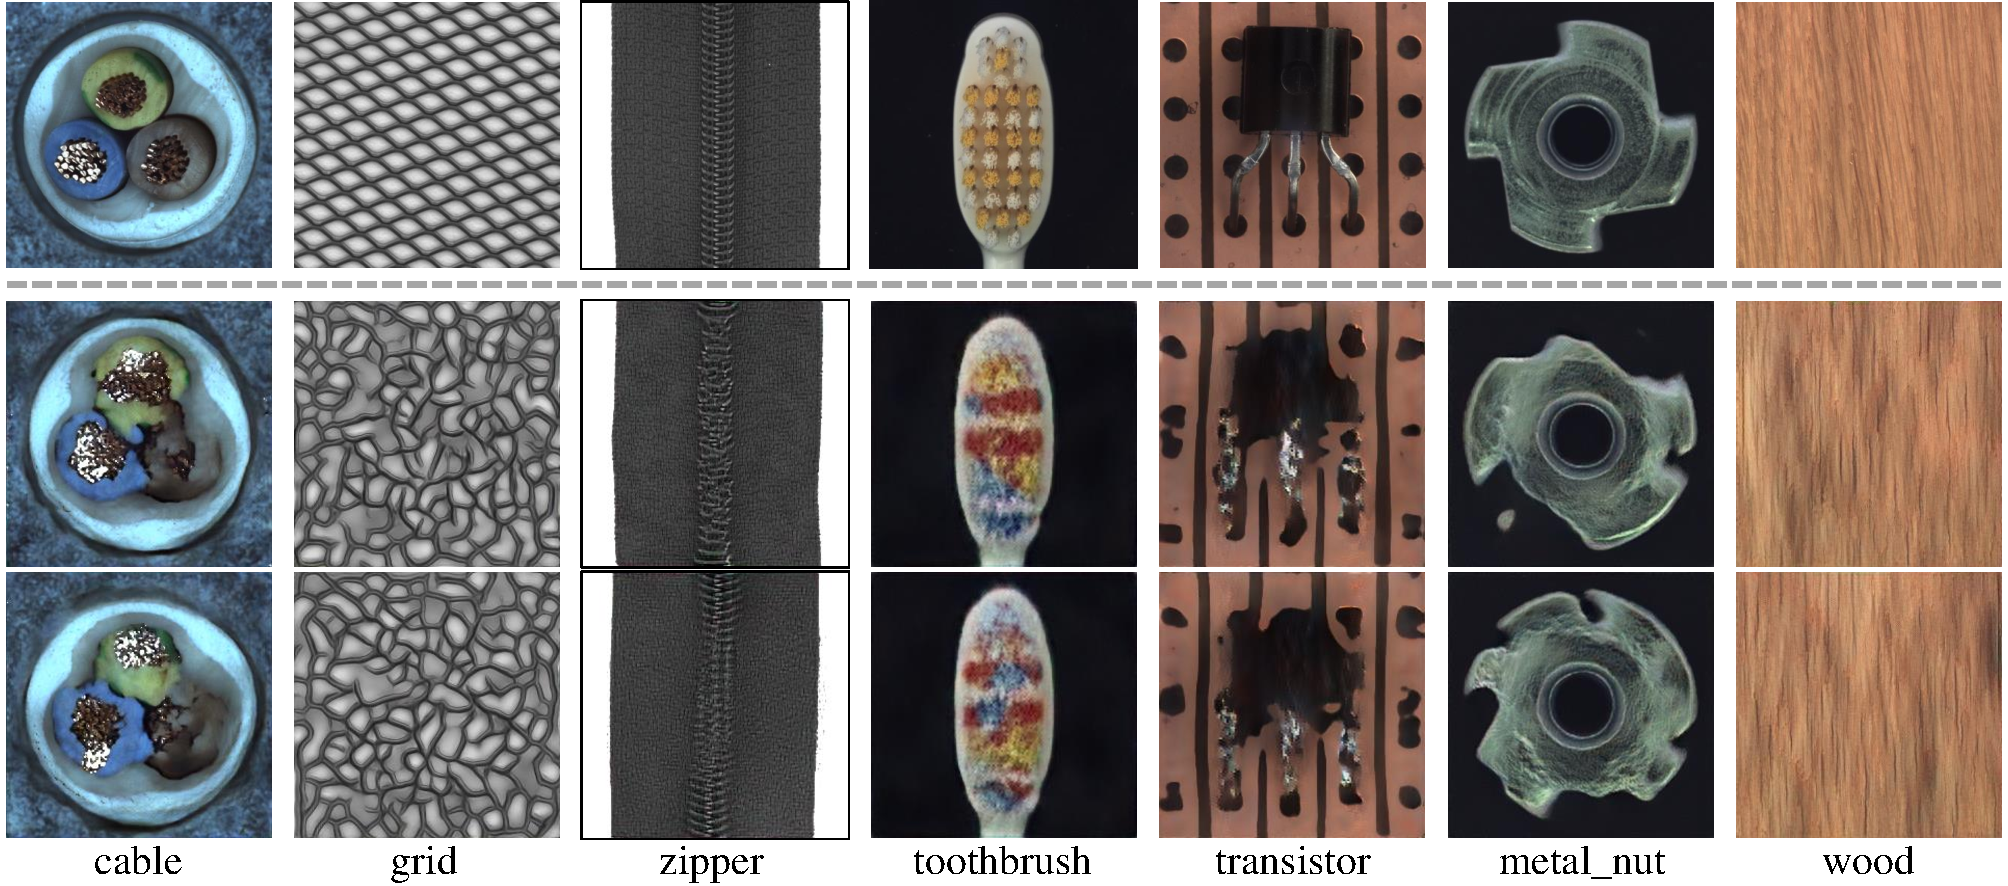
\includegraphics[width=0.7\linewidth]{images/mvtec_generation_results.pdf}
    \caption{Contrastive images generated by level-13 PatchDiff for MVTec AD~\cite{MVTecAD}. } 
    \label{fig: mvtec_generation}
\end{figure*}

\begin{table*}[!h]
    \centering
    % \footnotesize
    % \setlength{\belowcaptionskip}{0.2cm}
    % \setlength{\abovecaptionskip}{0.0cm}
    \renewcommand{\arraystretch}{1.2}
    \resizebox{\textwidth}{!}
    {
\begin{tabular}{cl|c|c|c|c|c|c|c|c}
\toprule
% \multicolumn{2}{c|}{Category} & \makecell[c]{IGD\\\tiny{\citealp{IGD}}} & \makecell[c]{PSVDD\\\tiny{\citealp{PSVDD}}} & \makecell[c]{FCDD\\\tiny{\citealp{FCDD}}} & \makecell[c]{CutPaste\\\tiny{\citealp{CutPaste}}} & \makecell[c]{NSA\\\tiny{\citealp{NSA}}} & \makecell[c]{DRAEM\\\tiny{\citealp{DRAEM}}} & \makecell[c]{DSR\\\tiny{\citealp{DSR}}} & \makecell[c]{GRAD\\\tiny{Ours}} \\ \midrule
\multicolumn{2}{c|}{Category}     & IGD & PSVDD & FCDD & CutPaste &NSA & DRAEM & DSR & GRAD \\ \midrule
\multirow{5}{*}{Texture} 
& carpet & (94.7, 82.8 ) & (92.9, 92.6) & (96.0, - ) & (93.1, 98.3) & (95.5, 95.6) & (95.5,97.0) & (-, \textbf{100.}) & (\textbf{96.5}, 98.2) \\
& grid & (97.7, 97.8 ) & (94.6, 100.) & (91.0, - ) & (\textbf{99.9}, 97.5) & (99.2, 99.9) & (99.7, 99.9) & (-, \textbf{100.}) & (97.2, \textbf{100.}) \\
& leather & (99.5, 95.8) & (90.9, 98.6) & (98.0, - ) & (\textbf{100.}, 99.5) & (99.5, 99.9) & (98.6, \textbf{100.}) & (-, \textbf{100.}) & (98.8, \textbf{100.}) \\
& tile & (78.0, 99.1) & (97.8, 91.4) & (91.0, - ) & (93.4, 90.5) & (\textbf{99.3}, \textbf{100.}) & (99.2, 99.6) & (-, \textbf{100.}) & (95.4, \textbf{100.}) \\
& wood & (89.1, 94.6) & (96.5, 90.8) & (88.0, - ) & (\textbf{98.6}, 95.5) & (90.7, 97.5) & (96.4, \textbf{99.1}) & (-, 96.3) & (87.2, 98.3) \\
\midrule
\multirow{10}{*}{Object} 
& bottle & (92.2, \textbf{100.}) & (98.6, 98.1) & (97.0, - ) & (98.3, 97.6) & (98.3, 97.7) & (\textbf{99.1}, 99.2) & (-, \textbf{100.}) & (96.5, \textbf{100.}) \\
& cable & (84.7, 90.6) & (90.3, 96.8) & (90.0, - ) & (80.6, 90.0) & (96.0, 94.5) & (94.7, 91.8) & (-, 93.8) & (\textbf{98.4}, \textbf{99.3}) \\
& capsule & (\textbf{97.7}, 91.5) & (76.7, 95.8) & (93.0, - ) & (96.2, 97.4) & (97.6, 95.2) & (94.3, \textbf{98.5}) & (-, 98.1) & (97.1, 96.4) \\
& hazelnut & (98.0, 99.7) & (92.0, 97.5) & (95.0, - ) & (97.3, 97.3) & (97.6, 94.7) & (\textbf{99.7}, \textbf{100.}) & (-, 95.6) & (96.6, 98.1) \\
& metal nut & (92.6, 91.3) & (94.0, 98.0) & (94.0, - ) & (99.3, 93.1) & (98.4, 98.7) & (\textbf{99.5}, 98.7) & (-, 98.5) & (93.7, \textbf{100.}) \\
& pill & (97.3, 87.3) & (86.1, 95.1) & (81.0, - ) & (92.4, 95.7) & (\textbf{98.5}, \textbf{99.2}) & (97.6, 98.9) & (-, 97.5) & (98.1, 95.7) \\
& screw & (97.0, 82.5) & (81.3, 95.7) & (86.0, - ) & (86.3, \textbf{96.7}) & (96.5, 90.2) & (97.6, 93.9) & (-, 96.2) & (\textbf{99.2}, 96.0) \\
& toothbrush & (97.7, 99.7) & (\textbf{100.}, 98.1) & (94.0, - ) & (98.3, 98.1) & (94.9, \textbf{100.}) & (98.1, \textbf{100.}) & (-, 99.7) & (98.0, 99.7) \\
& transistor & (84.4, 90.6) & (91.5, 97.0) & (88.0, - ) & (95.5, 93.0) & (88.0, 95.1) & (90.9, 93.1) & (-, 97.8) & (\textbf{97.8}, \textbf{100.}) \\
& zipper & (96.7, 97.0) & (97.9, 95.1) & (92.0, - ) & (\textbf{99.4}, 99.3) & (94.2, 99.8) & (98.9, \textbf{100.}) & (-, \textbf{100.}) & (98.3, 99.7) \\
\midrule
\multicolumn{2}{c|}{Average} & (93.1, 93.4) & (92.5, 93.2 ) & (92.1, 95.7) & (95.2, 96.0) & (96.3, 97.2) & (\textbf{97.3}, 98.0) & (-, 98.2) & (96.8, \textbf{98.7}) \\
\bottomrule
\end{tabular}}
\caption{Anomaly detection performance on MVTec AD dataset~\cite{MVTecAD}. Both pixel-level (left) and image-level (right) AUROC results are shown in each column. The best results are in bold.}
\label{tab: mvtec_main_detail}
\end{table*}

\subsection{Anomaly Detection and Localization}
In the main body, we exclusively present the averaged performance comparison on MVTec AD. In this section, we extend our analysis to provide a detailed result of the anomaly detection and localization performance across each individual sub-dataset within MVTec AD, and display anomaly maps on MVTec AD in Fig.~\ref{fig: main_mvtec_ad_results}. As shown in Table~\ref{tab: mvtec_main_detail}, we compare GRAD to IGD~\cite{IGD}, PSVDD~\cite{PSVDD}, FCDD~\cite{FCDD}, CutPaste~\cite{CutPaste}, NSA~\cite{NSA}, DRAEM~\cite{DRAEM}, and DSR~\cite{DSR}, all of which are independent of pretrained feature extractors. It is easy to find GRAD achieves a strong detection and localization of anomalies.  

\begin{figure*}[!h]
    \centering
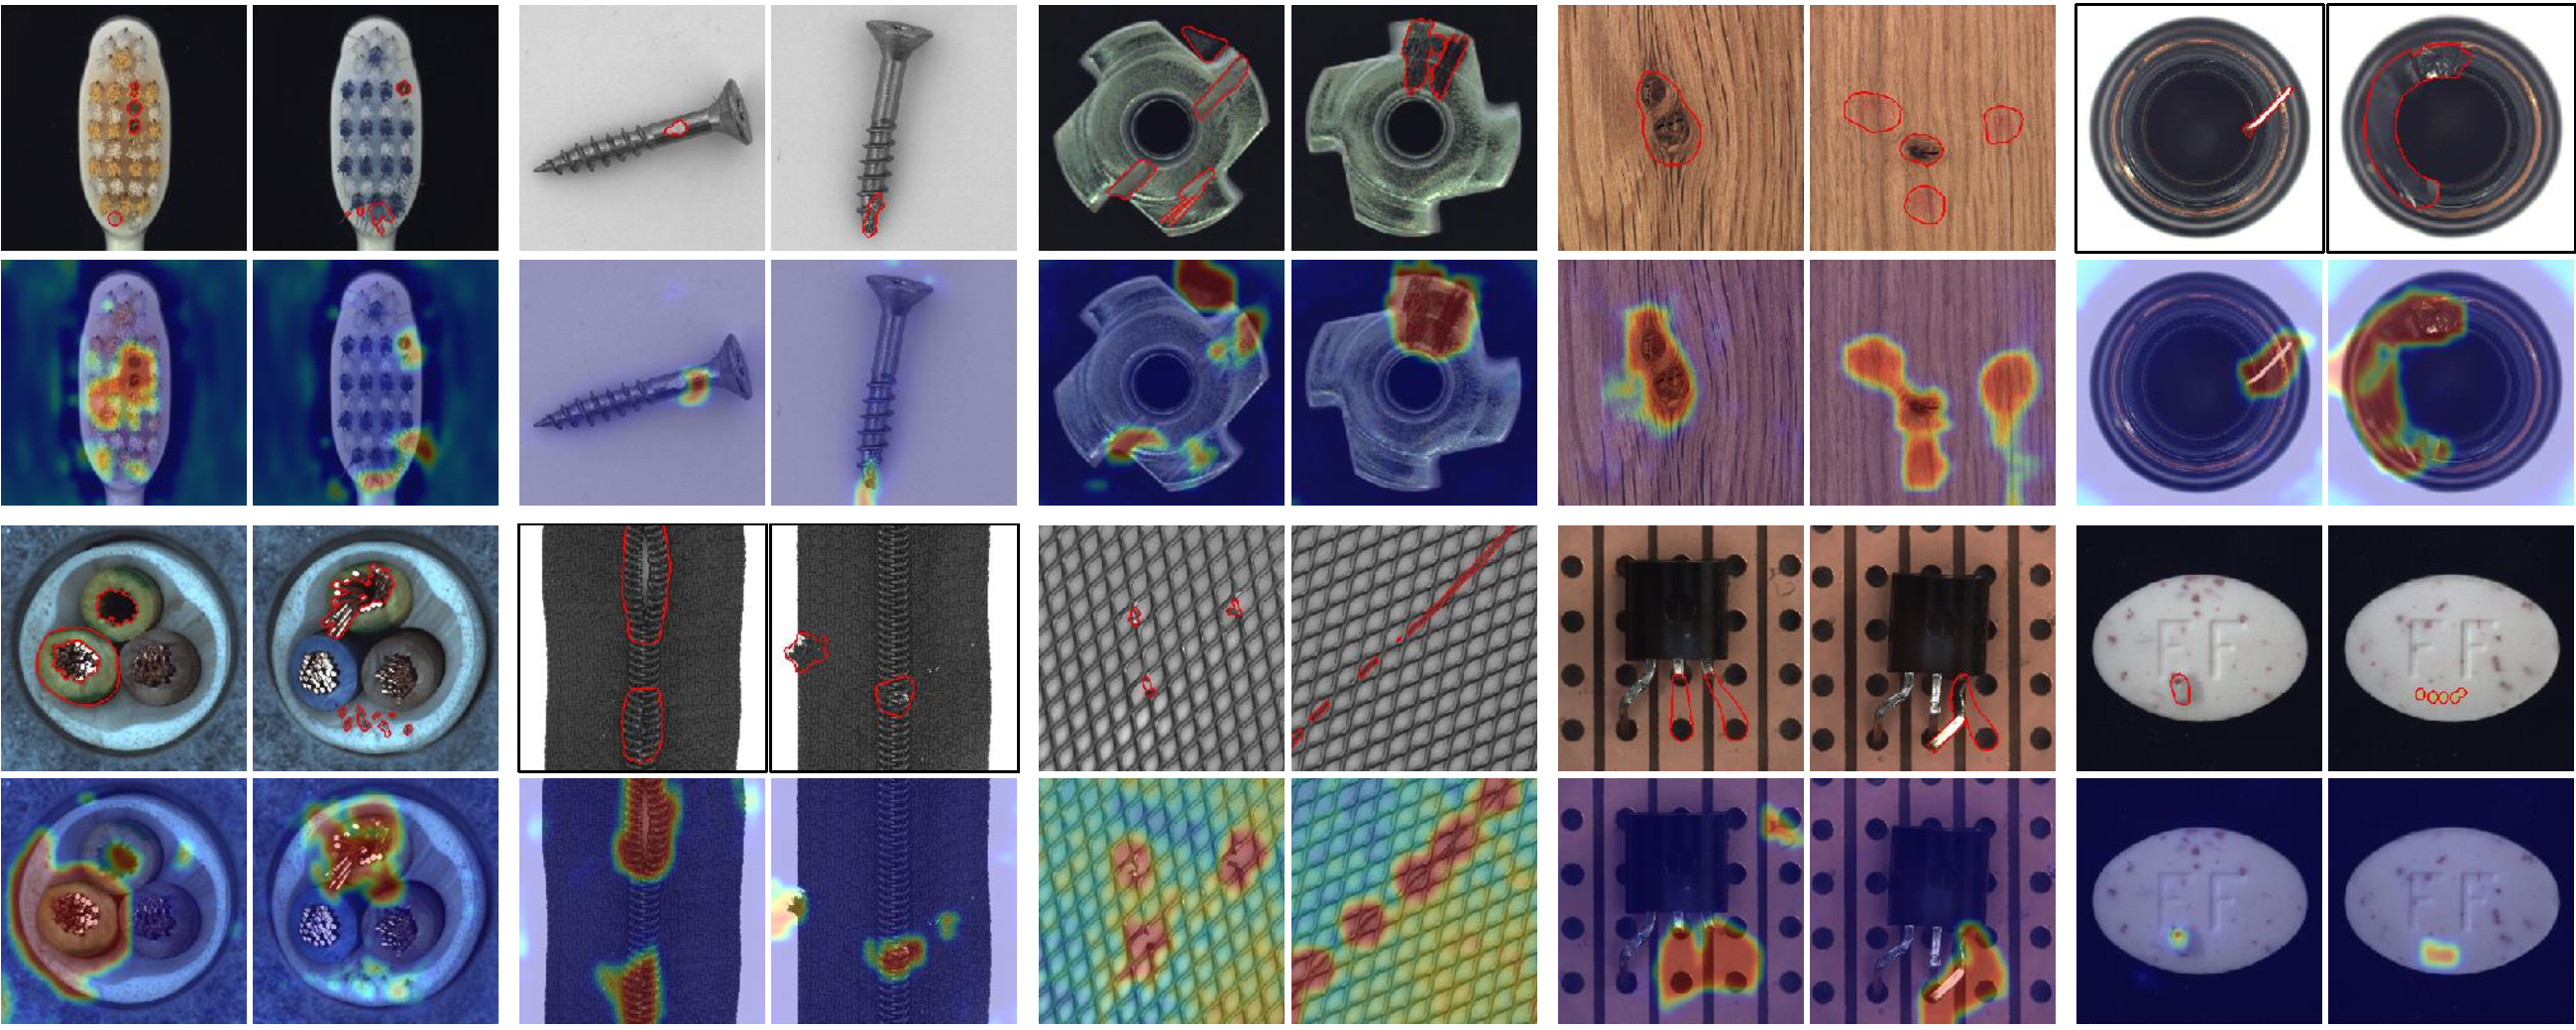
\includegraphics[width=0.9\linewidth]{images/mvtec_results.pdf}
    \caption{Defect localization results of GRAD on MVTec AD~\cite{MVTecAD}. } 
    \label{fig: main_mvtec_ad_results}
    % \vspace{-0.2cm}
\end{figure*}


% In addition, as shown in Table~\ref{tab:ablation_GRad_level}, we conduct an ablations study on selecting levels of patch-level detectors. It is easy to find that when integrating all three different levels of detectors, GRAD can achieve a strong performance for the detection of structural as well as logical anomalies.

% \begin{table}[!htbp]
% \centering
% \footnotesize
% \resizebox{0.3\textwidth}{!}{
% \begin{tabular}{ccc|c}
% \toprule
% \multicolumn{3}{c|}{Level Settings}& Image-level \\
% 136 & 68 & 34  & AUROC\\
% \midrule
% \checkmark &   \ding{55} & \ding{55}   &  85.2   \\
% \ding{55}& \checkmark & \ding{55} & 85.4 \\
% \ding{55}&\ding{55} & \checkmark & 75.1\\
% \checkmark & \checkmark & \ding{55}   &  86.8     \\ %
% \checkmark &   \ding{55} & \checkmark   &  86.4   \\
% \ding{55} & \checkmark & \checkmark  & 86.2 \\
% \checkmark & \checkmark & \checkmark &  \textbf{87.5}  \\
% \bottomrule
% \end{tabular}}
% \caption{Ablation study on detector levels. Detection AUROC results on MVTec LOCO dataset. The best results are in bold.}
% \label{tab:ablation_GRad_level}
% \end{table}



% \bibliography{aaai24}
% \bibliographystyle{aaai24}

% \end{document}

}

\end{document}